%
% A header that lets you compile a chapter by itself, or inside a larger document.
% Adapted from http://stackoverflow.com/questions/3655454/conditional-import-in-latex
%
%
%Use \inbpdocument and \outbpdocument in your individual files, in place of \begin{document} and \end{document}. In your main file, put in a \def \ismaindoc {} before including or importing anything.
%
% David Duvenaud
% June 2011
% 
% ======================================
%
%


\ifx\ismaindoc\undefined
	\newcommand{\inbpdocument}{
		\def \ismaindoc {}
		% Use this header if we are compiling by ourselves.
		\documentclass[a4paper,11pt,authoryear,index]{common/PhDThesisPSnPDF}
		
%\usepackage{draftwatermark}
%\SetWatermarkLightness{0.95}

% ******************************************************************************
% ****************************** Custom Margin *********************************

% Add `custommargin' in the document class options to use this section
% Set {innerside margin / outerside margin / topmargin / bottom margin}  and
% other page dimensions

\ifsetMargin
\else
    \RequirePackage[left=37mm,right=30mm,top=35mm,bottom=30mm]{geometry}
    \setFancyHdr % To apply fancy header after geometry package is loaded
\fi


%\chead{Unfinished draft}
%\cfoot{\texttt{Unfinished draft - compiled on \today{} at \currenttime}}

% *****************************************************************************
% ******************* Fonts (like different typewriter fonts etc.)*************

% Add `customfont' in the document class option to use this section

\ifsetFont
\else
    % Set your custom font here and use `customfont' in options. Leave empty to
    % load computer modern font (default LaTeX font).  

    \RequirePackage{libertine} 
\fi

% *****************************************************************************
% *************************** Bibliography  and References ********************

%\usepackage{cleveref} %Referencing without need to explicitly state fig /table

% Add `custombib' in the document class option to use this section
\ifsetBib % True, Bibliography option is chosen in class options
\else % If custom bibliography style chosen then load bibstyle here

   \RequirePackage[square, sort, numbers, authoryear]{natbib} % CustomBib

% If you would like to use biblatex for your reference management, as opposed to the default `natbibpackage` pass the option `custombib` in the document class. Comment out the previous line to make sure you don't load the natbib package. Uncomment the following lines and specify the location of references.bib file

% \RequirePackage[backend=biber, style=numeric-comp, citestyle=numeric, sorting=nty, natbib=true]{biblatex}
% \bibliography{References/references} %Location of references.bib only for biblatex

\fi


% changes the default name `Bibliography` -> `References'
\renewcommand{\bibname}{References}


% *****************************************************************************
% *************** Changing the Visual Style of Chapter Headings ***************
% Uncomment the section below. Requires titlesec package.

%\RequirePackage{titlesec}
%\newcommand{\PreContentTitleFormat}{\titleformat{\chapter}[display]{\scshape\Large}
%{\Large\filleft{\chaptertitlename} \Huge\thechapter}
%{1ex}{}
%[\vspace{1ex}\titlerule]}
%\newcommand{\ContentTitleFormat}{\titleformat{\chapter}[display]{\scshape\huge}
%{\Large\filleft{\chaptertitlename} \Huge\thechapter}{1ex}
%{\titlerule\vspace{1ex}\filright}
%[\vspace{1ex}\titlerule]}
%\newcommand{\PostContentTitleFormat}{\PreContentTitleFormat}
%\PreContentTitleFormat


% *****************************************************************************
% **************************** Custom Packages ********************************
% *****************************************************************************


% ************************* Algorithms and Pseudocode **************************

%\usepackage{algpseudocode} 


% ********************Captions and Hyperreferencing / URL **********************

% Captions: This makes captions of figures use a boldfaced small font. 
%\RequirePackage[small,bf]{caption}

\RequirePackage[labelsep=space,tableposition=top]{caption} 
%\renewcommand{\figurename}{Figure} %to support older versions of captions.sty
\captionsetup{belowskip=12pt,aboveskip=4pt}

% ************************ Formatting / Footnote *******************************

%\usepackage[perpage]{footmisc} %Range of footnote options 


% ****************************** Line Numbers **********************************

%\RequirePackage{lineno}
%\linenumbers

% ************************** Graphics and figures *****************************

%\usepackage{rotating}
%\usepackage{wrapfig}
%\usepackage{float}
\usepackage{subfig} %note: subfig must be included after the `caption` package. 


% ********************************* Table **************************************

%\usepackage{longtable}
%\usepackage{multicol}
%\usepackage{multirow}
%\usepackage{tabularx}


% ***************************** Math and SI Units ******************************

\usepackage{amsfonts}
\usepackage{amsmath}
\usepackage{amssymb}
%\usepackage{siunitx} % use this package module for SI units


% ******************************************************************************
% ************************* User Defined Commands ******************************
% ******************************************************************************

% *********** To change the name of Table of Contents / LOF and LOT ************

%\renewcommand{\contentsname}{My Table of Contents}
%\renewcommand{\listfigurename}{List of figures}
%\renewcommand{\listtablename}{List of tables}


% ********************** TOC depth and numbering depth *************************

\setcounter{secnumdepth}{2}
\setcounter{tocdepth}{2}

% ******************************* Nomenclature *********************************

% To change the name of the Nomenclature section, uncomment the following line

%\renewcommand{\nomname}{Symbols}


% ********************************* Appendix ***********************************

% The default value of both \appendixtocname and \appendixpagename is `Appendices'. These names can all be changed via: 

%\renewcommand{\appendixtocname}{List of appendices}
%\renewcommand{\appendixname}{Appndx}

		% All my custom preamble stuff.  Shouldn't overlap with anything in official-preamble


% Paths to figure and table directories.
\newcommand{\symmetryfigsdir}{figures/symmetries}
\newcommand{\topologyfiguresdir}{figures/topology}
\newcommand{\infinitefiguresdir}{figures/infinite}
\newcommand{\grammarfiguresdir}{figures/grammar}
\newcommand{\introfigsdir}{figures/intro}
\newcommand{\gplvmfiguresdir}{figures/gplvm}
\newcommand{\warpedfiguresdir}{figures/warped-mixtures}
\newcommand{\deeplimitsfiguresdir}{figures/deep-limits}
\newcommand{\quadraturefigsdir}{figures/quadrature}
\newcommand{\additivefigsdir}{figures/additive}
\newcommand{\decompfigsdir}{figures/decomp}
\newcommand{\examplefigsdir}{figures/worked-example}


\usepackage{bm}  % for warped mixtures - is this necessary?
\usepackage{booktabs}
\usepackage{tabularx}
\usepackage{multirow}
\usepackage{datetime}
\renewcommand{\tabularxcolumn}[1]{>{\arraybackslash}m{#1}}
\usepackage{relsize}
\usepackage{graphicx}
\usepackage{amsmath,amssymb,textcomp}
\usepackage{nicefrac}
\usepackage{amsthm}
\usepackage{tikz}
\usetikzlibrary{arrows}
\usetikzlibrary{calc}
\usepackage{nth}
\usepackage{rotating}
\usepackage{array}
\usepackage{fp}
\usepackage[hyperpageref]{backref}
\def\foo{\hspace{\fill}\mbox{}\linebreak[0]\hspace*{\fill}}
\renewcommand*{\backref}[1]{}
\renewcommand*{\backrefalt}[4]{%
\ifcase #1 %
%
\or
\foo(page #2)%
\else
\foo(pages #2)%
\fi
}

\usepackage{cleveref}
\crefname{equation}{equation}{equations}


%% For submission, make all render blank.
%%%%%%%%%%%%%%%%%%%%%%%%%%%%%%%%%%%%%%%%%%%%%%%%%%%%%%%%%%
%%%% EDITING HELPER FUNCTIONS  %%%%%%%%%%%%%%%%%%%%%%%%%%%
%%%%%%%%%%%%%%%%%%%%%%%%%%%%%%%%%%%%%%%%%%%%%%%%%%%%%%%%%%

%% NA: needs attention (rough writing whose correctness needs to be verified)
%% TBD: instructions for how to fix a gap ("Describe the propagation by ...")
%% PROBLEM: bug or missing crucial bit 

%% use \fXXX versions of these macros to put additional explanation into a footnote.  
%% The idea is that we don't want to interrupt the flow of the paper or make it 
%% impossible to read because there are a bunch of comments.

%% NA's (and TBDs, those less crucially) should be written so 
%% that they flow with the text.

\definecolor{WowColor}{rgb}{.75,0,.75}
\definecolor{SubtleColor}{rgb}{0,0,.50}

% inline
\newcommand{\NA}[1]{\textcolor{SubtleColor}{ {\tiny \bf ($\star$)} #1}}
\newcommand{\LATER}[1]{\textcolor{SubtleColor}{ {\tiny \bf ($\dagger$)} #1}}
\newcommand{\TBD}[1]{\textcolor{SubtleColor}{ {\tiny \bf (!)} #1}}
\newcommand{\PROBLEM}[1]{\textcolor{WowColor}{ {\bf (!!)} {\bf #1}}}

% as margin notes

\newcounter{margincounter}
\newcommand{\displaycounter}{{\arabic{margincounter}}}
\newcommand{\incdisplaycounter}{{\stepcounter{margincounter}\arabic{margincounter}}}

\newcommand{\fTBD}[1]{\textcolor{SubtleColor}{$\,^{(\incdisplaycounter)}$}\marginpar{\tiny\textcolor{SubtleColor}{ {\tiny $(\displaycounter)$} #1}}}

\newcommand{\fPROBLEM}[1]{\textcolor{WowColor}{$\,^{((\incdisplaycounter))}$}\marginpar{\tiny\textcolor{WowColor}{ {\bf $\mathbf{((\displaycounter))}$} {\bf #1}}}}

\newcommand{\fLATER}[1]{\textcolor{SubtleColor}{$\,^{(\incdisplaycounter\dagger)}$}\marginpar{\tiny\textcolor{SubtleColor}{ {\tiny $(\displaycounter\dagger)$} #1}}}

%\renewcommand{\LATER}[1]{}
%\renewcommand{\fLATER}[1]{}
%\renewcommand{\TBD}[1]{}
%\renewcommand{\fTBD}[1]{}
%\renewcommand{\PROBLEM}[1]{}
%\renewcommand{\fPROBLEM}[1]{}
%\renewcommand{\NA}[1]{}


% HUMBLE WORDS: shown slightly smaller when in normal text
% Thanks to Christian Steinruecken!

% HUMBLE WORDS: shown slightly smaller when in normal text
%
\makeatletter%
%\def\@humbleformat#1{{\fontsize{}{1em}\selectfont #1}}
%\def\@humbleformat#1{\textsmaller{#1}}%
\newlength{\nonHumbleHeight}
\def\@humbleformat#1{{\settoheight{\nonHumbleHeight}{#1}\resizebox{!}{0.94\nonHumbleHeight}{#1}}}%
\def\@idxhumbleformat#1{{\relscale{0.95}{#1}}}%
%\def\@humbleformat#1{{#1}}%
\def\declareHumble#1#2{%
  \expandafter\def\csname #1\endcsname{\@humbleformat{#2}}%
  \expandafter\def\csname s#1\endcsname{{#2}}%
  \expandafter\def\csname idx#1\endcsname{{\@idxhumbleformat{#2}}}%
}%
\def\humble#1{\@humbleformat{#1}}%
\def\idxhumble#1{\@idxhumbleformat{#1}}%
\makeatother%

% Convenient indexing for humble abbreviations
\def\humbleindex#1#2{\index{#1@\idxhumble{#1}}}



% TODO: Clean up duplicates
\declareHumble{ANOVA}{ANOVA}
\declareHumble{ARD}{ARD}
\declareHumble{BIC}{BIC}
\declareHumble{BMC}{BMC}
\declareHumble{bq}{BQ}
\declareHumble{CRP}{CRP}
\declareHumble{dirpro}{DP}
\declareHumble{HDMR}{HDMR}
\declareHumble{GAM}{GAM}
\declareHumble{GEM}{GEM}
\declareHumble{GMM}{GMM}
\declareHumble{gplvm}{GP-LVM}
\declareHumble{gpml}{GPML}
\declareHumble{GPML}{GPML}
\declareHumble{gprn}{GPRN}
\declareHumble{gpt}{GP}
\declareHumble{gp}{GP}
\declareHumble{HKL}{HKL}
\declareHumble{HMC}{HMC}
\declareHumble{ibp}{IBP}
\declareHumble{iGMM}{iGMM}
\declareHumble{iwmm}{iWMM}
\declareHumble{kCP}{CP}
\declareHumble{kCW}{CW}
\declareHumble{kC}{C}
\declareHumble{KDE}{KDE}
\declareHumble{kLin}{Lin}
\declareHumble{KPCA}{KPCA}
\declareHumble{kPer}{Per}
\declareHumble{kRQ}{RQ}
\declareHumble{kSE}{SE}
\declareHumble{kWN}{WN}
\declareHumble{Lin}{Lin}
\declareHumble{LBFGS}{L-BFGS}
\declareHumble{mcmc}{MCMC}
\declareHumble{MKL}{MKL}
\declareHumble{MLP}{MLP}
\declareHumble{MSE}{MSE}
\declareHumble{Per}{Per}
\declareHumble{RMSE}{RMSE}
\declareHumble{RQ}{RQ}
\declareHumble{SBQ}{SBQ}
\declareHumble{seard}{SE-ARD}
\declareHumble{sefull}{SE-\textnormal{full}}
\declareHumble{SEGP}{SE-GP}
\declareHumble{SE}{SE}
\declareHumble{SNR}{SNR}
\declareHumble{SSANOVA}{SS-ANOVA}
\declareHumble{SVM}{SVM}

\newcommand{\kSig}{\boldsymbol\sigma}

\def\subexpr{{\cal S}}
\def\baseker{{\cal B}}
\def\numWinners{k}

\def\ie{i.e.\ }
\def\eg{e.g.\ }
\def\etc{etc.\ }
\let\oldemptyset\emptyset
\let\emptyset 0




% Unify notation between neural-net land and GP-land.
\newcommand{\hphi}{h}
\newcommand{\hPhi}{\vh}
\newcommand{\walpha}{w}
\newcommand{\wboldalpha}{\bw}
\newcommand{\wcapalpha}{\vW}
\newcommand{\lengthscale}{w}

\newcommand{\layerindex}{\ell}



\newcommand{\gpdrawbox}[1]{
\setlength\fboxsep{0pt}
\hspace{-0.15in} 
\fbox{
\includegraphics[width=0.464\columnwidth]{\deeplimitsfiguresdir/deep_draws/deep_gp_sample_layer_#1}
}}



\newcommand{\procedurename}{ABCD}
\newcommand{\genText}[1]{{\sf #1}}



\newcommand{\asdf}{$^{\textnormal{th}}$}

\newcommand{\binarysum}{\sum_{\bf{x} \in \{0,1\}^D}}
\newcommand{\expect}{\mathbb{E}}
\newcommand{\expectargs}[2]{\mathbb{E}_{#1} \left[ {#2} \right]}
\newcommand{\var}{\mathbb{V}}
\newcommand{\varianceargs}[2]{\mathbb{V}_{#1} \left[ {#2} \right]}
\newcommand{\cov}{\operatorname{cov}}
\newcommand{\Cov}{\operatorname{Cov}}
\newcommand{\covargs}[2]{\cov \left[ {#1}, {#2} \right]}
\newcommand{\variance}{\mathbb{V}}
\newcommand{\vecop}[1]{\operatorname{vec} \left( {#1} \right)}

\newcommand{\covarianceargs}[2]{\Cov_{#1} \left[ {#2} \right]}
\newcommand{\colvec}[2]{\left[ \begin{array}{c} {#1} \\ {#2} \end{array} \right]}
\newcommand{\tbtmat}[4]{\left[ \begin{array}{cc} {#1} & {#2} \\ {#3} & {#4} \end{array} \right]}

%\newcommand{\covskinny}[2]{\var\!\left(#1\middle\vert#2\right)} 

\newcommand{\acro}[1]{{\humble{#1}}}
%\newcommand{\vect}[1]{\boldsymbol{#1}}
\newcommand{\vect}[1]{{\bf{#1}}}
\newcommand{\mat}[1]{\mathbf{#1}}
\newcommand{\pderiv}[2]{\frac{\partial #1}{\partial #2}}
\newcommand{\npderiv}[2]{\nicefrac{\partial #1}{\partial #2}}

\newcommand{\pha}{^{\phantom{:}}}

\newcommand{\argmin}{\operatornamewithlimits{argmin}}
\newcommand{\argmax}{\operatornamewithlimits{argmax}}

% The following designed for probabilities with long arguments

\newcommand{\Prob}[2]{P\!\left(\,#1\;\middle\vert\;#2\,\right)}
\newcommand{\ProbF}[3]{P\!\left(\,#1\!=\!#2\;\middle\vert\;#3\,\right)}
\newcommand{\p}[2]{p\!\left(#1\middle\vert#2\right)}
\newcommand{\po}[1]{p\!\left(#1\right)}
\newcommand{\pF}[3]{p\!\left(\,#1\!=\!#2\;\middle\vert\;#3\,\right)} 
\newcommand{\mean}[2]{{m}\!\left(#1\middle\vert#2\right)}



\newcommand{\valpha}{\boldsymbol{\alpha}}
\newcommand{\va}{\vect{a}}
\newcommand{\vA}{\vect{A}}
\newcommand{\vB}{\mat{B}}
\newcommand{\vb}{\vect{b}}
\newcommand{\vC}{\mat{C}}
\newcommand{\vc}{\vect{c}}
\newcommand{\vecf}{\boldsymbol{f}}
\newcommand{\vell}{\vect{\ell}}
\newcommand{\vepsilon}{\boldsymbol{\epsilon}}
\newcommand{\veps}{\boldsymbol{\epsilon}}
\newcommand{\ve}{\boldsymbol{\epsilon}}
\newcommand{\vf}{\vecf}
\newcommand{\vg}{\vect{g}}
\newcommand{\vh}{\vect{h}}
\newcommand{\vI}{\mat{I}}
\newcommand{\vK}{\mat{K}}
\newcommand{\vk}{\vect{k}}
\newcommand{\vL}{\mat{L}}
\newcommand{\vl}{\vect{l}}
\newcommand{\vmu}{\boldsymbol{\mu}}
\newcommand{\vone}{\vect{1}}
\newcommand{\vphi}{\boldsymbol{\phi}}
\newcommand{\vpi}{\boldsymbol{\pi}}
\newcommand{\vq}{\vect{q}}
\newcommand{\vR}{\mat{R}}
\newcommand{\vr}{\vect{r}}
\newcommand{\vsigma}{\boldsymbol{\sigma}}
\newcommand{\vSigma}{\mat{\Sigma}}
\newcommand{\vS}{\mat{S}}
\newcommand{\vs}{\vect{s}}
\newcommand{\vtheta}{\boldsymbol{\theta}}
\newcommand{\vu}{\vect{u}}
\newcommand{\vV}{\mat{V}}
\newcommand{\vW}{\mat{W}}
\newcommand{\vw}{\vect{w}}
\newcommand{\vX}{\mat{X}}
\newcommand{\vx}{\vect{x}}
\newcommand{\vY}{\mat{Y}}
\newcommand{\vy}{\vect{y}}
\newcommand{\vzero}{\vect{0}}
\newcommand{\vZ}{\mat{Z}}
\newcommand{\vz}{\vect{z}}


\newcommand{\netweights}{\alpha}
\newcommand{\vnetweights}{\valpha}

\newcommand{\He}{\mathcal{H}}
\newcommand{\normx}[2]{\left\|#1\right\|_{#2}}
\newcommand{\Hnorm}[1]{\normx{#1}{\He}}
\newcommand{\mmd}{{\rm MMD}}


\newcommand{\mf}{\bar{\vf}}

%\newcommand{\mf}{\mu} %{\bar{\ell}}
\newcommand{\lf}{f} % Likelihood function
\newcommand{\st}{_\star}

% from simpler log-bq writeup
\newcommand{\lftwo}{{\log \ell}}
\newcommand{\mftwo}{{\bar \ell}}
\newcommand{\loggp}{{\log\acro{GP}}}%| \bX, \vy )}}
\newcommand{\loggpdist}{{\acro{GP}(\lftwo)}}%| \vX, \vy )}}


\newcommand{\inv}{^{{\mathsmaller{-1}}}}
\newcommand{\tohalf}{^{{\mathsmaller{\nicefrac{1}{2}}}}}

\newcommand{\Normal}{\mathcal{N}}
\newcommand{\N}[3]{\mathcal{N}\!\left(#1 \middle| #2,#3\right)}
\newcommand{\Nt}[2]{\mathcal{N}\!\left(#1,#2\right)}
\newcommand{\NT}[2]{\mathcal{N}\!\left(#1,#2\right)}
\newcommand{\GPdist}[3]{\mathcal{GP}\!\left(#1 \, \middle| \, #2, #3 \right)}
\newcommand{\bN}[3]{\mathcal{N}\big(#1 \middle| #2,#3\big)}
\newcommand{\boldN}[3]{\text{\textbf{\mathcal{N}}}\big(#1;#2,#3\big)}
\newcommand{\ones}[1]{\mat{1}_{#1}}
\newcommand{\eye}[1]{\mat{E}_{#1}}
\newcommand{\tra}{^{\mathsf{T}}}
%\newcommand{\tra}{^{\top}}
%\mathsf{T}
\newcommand{\trace}{\operatorname{tr}}
\newcommand{\shift}{\operatorname{shift}}
\renewcommand{\mod}{\operatorname{mod}}
\newcommand{\deq}{:=}
\newcommand{\oneofk}{\operatorname{one-of-k}}
%\newcommand{\degree}{^\circ}

\newcommand{\GPt}[2]{\mathcal{GP}\!\left(#1,#2\right)}
%\newcommand{\GPt}[2]{\gp\!\left(#1,#2\right)}

\DeclareMathOperator{\tr}{tr}
\DeclareMathOperator{\chol}{chol}
\DeclareMathOperator{\diag}{diag}

\newenvironment{narrow}[2]{%
  \begin{list}{}{%
  \setlength{\topsep}{0pt}%
  \setlength{\leftmargin}{#1}%
  \setlength{\rightmargin}{#2}%
  \setlength{\listparindent}{\parindent}%
  \setlength{\itemindent}{\parindent}%
  \setlength{\parsep}{\parskip}}%
\item[]}{\end{list}}



\newcommand{\dist}{\ \sim\ }
\def\given{\,|\,}

% Table stuff
\newcolumntype{C}[1]{>{\centering\let\newline\\\arraybackslash\hspace{0pt}}m{#1}}
\newcolumntype{L}[1]{>{\raggedright\let\newline\\\arraybackslash\hspace{0pt}}m{#1}}
\newcolumntype{R}[1]{>{\raggedleft\let\newline\\\arraybackslash\hspace{0pt}}m{#1}}


\def\ie{i.e.\ }
\def\eg{e.g.\ }
\def\iid{i.i.d.\ }
%\def\simiid{\sim_{\mbox{\tiny iid}}}
\def\simiid{\overset{\mbox{\tiny iid}}{\sim}}
\def\simind{\overset{\mbox{\tiny \textnormal{ind}}}{\sim}}
\def\eqdist{\stackrel{\mbox{\tiny d}}{=}}
%\newcommand{\distas}[1]{\mathbin{\overset{#1}{\kern \z@ \sim}}}
%TODO: fix this - it worked outside the thesis!
\newcommand{\distas}[1]{\mathbin{\overset{#1}{\sim}}}

\def\Reals{\mathbb{R}}

\def\Uniform{\mbox{\rm Uniform}}
\def\Bernoulli{\mbox{\rm Bernoulli}}
\def\GP{\mathcal{GP}}
\def\GPLVM{\mathcal{GP-LVM}}




% Kernel stuff

\def\iva{\vect{\inputVar}}
\def\ivaone{\inputVar}
\def\inputVar{x}
\def\InputVar{X}
\def\InputSpace{\mathcal{X}}
\def\outputVar{y}
\def\OutputSpace{\mathcal{Y}}
\def\function{f}
\def\kernel{k}
\def\KernelMatrix{K}
\def\SumKernel{\sum}
\def\ProductKernel{\prod}
\def\expression{e}
\def\feat{\vh}

\newcommand{\kerntimes}{ \! \times \!}
\newcommand{\kernplus}{ \, + \,}


% Proof stuff
\theoremstyle{plain}
\newtheorem{theorem}{Theorem}[section]
\newtheorem{lemma}[theorem]{Lemma}
\newtheorem{prop}[theorem]{Proposition}
\newtheorem{proposition}{Proposition}
\newtheorem*{cor}{Corollary}

% For infinite bq
\newcommand{\iv}{\theta}
\newcommand{\viv}{\vtheta}

% For intro chapter
\newcommand{\funcval}{\vf(\vX)}
\newcommand{\testpoint}{{\vx^\star}}

\newcommand{\underwrite}[2]{{\underbrace{#1}_{\textnormal{#2}}}}



% For kernel figures
\newcommand{\fhbig}{2cm}%
\newcommand{\fwbig}{3cm}%
\newcommand{\kernpic}[1]{\includegraphics[height=\fhbig,width=\fwbig]{\grammarfiguresdir/structure_examples/#1}}%
\newcommand{\kernpicr}[1]{\rotatebox{90}{\includegraphics[height=\fwbig,width=\fhbig]{\grammarfiguresdir/structure_examples/#1}}}%
\newcommand{\addkernpic}[1]{{\includegraphics[height=\fhbig,width=\fwbig]{\grammarfiguresdir/additive_multi_d/#1}}}%
\newcommand{\largeplus}{\tabbox{{\Large+}}}%
\newcommand{\largeeq}{\tabbox{{\Large=}}}%
\newcommand{\largetimes}{\tabbox{{\Large$\times$}}}%
\newcommand{\fixedx}{$x$ (with $x' = 1$)}%


		% ************************ Thesis Information & Meta-data **********************

%% The title of the thesis
%\title{Structured Gaussian Process Models} 
%\title{Automatic Model Construction \\ through \\ Structured Gaussian Processes}
%\title{Automatic Model-Building \\ through \\ Structured Gaussian Processes}
%\title{Automatic Modeling \\ with \\ Structured Gaussian Processes}    
\title{Automatic Model Construction \\ with Gaussian Processes}
%\title{Automatic Model Construction}
%\title{Automating Statistical Model Construction}


%\texorpdfstring is used for PDF metadata. Usage:
%\texorpdfstring{LaTeX_Version}{PDF Version (non-latex)} eg.,
%\texorpdfstring{$sigma$}{sigma}

%% The full name of the author
\author{David Kristjanson Duvenaud}

%% Department (eg. Department of Engineering, Maths, Physics)
%\dept{Department of Engineering}

%% University and Crest
\university{University of Cambridge}
\crest{
\includegraphics[width=0.25\textwidth]{University_Crest}}

%% You can redefine the submission text:
% Default as per the University guidelines: This dissertation is submitted for
% the degree of Doctor of Philosophy
%\renewcommand{\submissiontext}{change the default text here if needed}

%% Full title of the Degree 
\degree{Doctor of Philosophy}
 
%% College affiliation (optional)
\college{Pembroke College}

%% Submission date
\degreedate{June 2014} 

%% Meta information
\subject{LaTeX} \keywords{{LaTeX} {PhD Thesis} {Engineering} {University of Cambridge}}



		\begin{document}
	}	
	\newcommand{\outbpdocument}[1]{

		% Fake chapters so references aren't broken
\label{ch:intro}                
\label{ch:kernels}
\label{ch:grammar}
\label{ch:description}
\label{ch:additive}
\label{ch:deeplimits}
\label{ch:discussion}
		%\bibliographystyle{common/CUEDthesis}
		\bibliographystyle{plainnat}
		\bibliography{references.bib}
		\end{document}
	}	
\else
	%If we're inside another document, no need to re-start the document.
	\ifx\inbpdocument\undefined
		\newcommand{\inbpdocument}{}
		\newcommand{\outbpdocument}[1]{}
	\fi
\fi

\inbpdocument

\chapter{Expressing Structure through Kernels}
\label{ch:kernels}





Kernels specify similarity between function values of two objects, not between similarity of objects



%Kernel functions $\kernel : \InputSpace \times \InputSpace \to \Reals$ can be used to define a measure of similarity between two points $\inputVar, \inputVar'$ in some space $\InputSpace$.
%\fTBD{Define $\GP\sim\dots$ here?}
Gaussian process models use a kernel to define the covariance between any two function values: ${\textrm{Cov}(\outputVar, \outputVar') = \kernel(\inputVar,\inputVar')}$.
%The kernel determines which sorts of structures the model places most of its probability mass upon, and in effect determines the generalization properties of the model.
The kernel specifies which structures are likely under the \gp{} prior, which in turn determines the generalization properties of the model.
%The kernel, $\kernel$, must define a valid covariance function\fTBD{expand me}; when this is the case $\kernel$ is said to be positive semi-definite (PSD).
%\fTBD{RBG: we should make the distinction between kernels and kernel families, and then use it consistently}
%
%Examples of commonly used kernels include squared exponential (SE), periodic (Per) and linear kernels (Lin) defined below\fTBD{If we add RQ then we have everything in one place}
%\begin{eqnarray}
%\kernel_\textrm{SE}(\inputVar, \inputVar') = & \sigma^2\exp\left(-\frac{(\inputVar - \inputVar')^2}{2\ell^2}\right) \\
%\kernel_\textrm{Per}(\inputVar, \inputVar') = & \sigma^2\exp\left(-\frac{2\sin^2(\pi|\inputVar - \inputVar'|/p)}{\ell^2}\right) \\
%\kernel_\textrm{Lin}(\inputVar, \inputVar') = & \sigma_b^2 + \sigma_v^2(\inputVar - \ell)(\inputVar' - \ell).
%\end{eqnarray}
%
In this section, we review the ways in which kernel families\footnotemark can be composed to express diverse priors over functions. 
\footnotetext{When unclear from context, we use `kernel family' to refer to the parametric forms of the functions given in the appendix. A kernel is a kernel family with all of the parameters specified.}  

There has been significant work on constructing \gp{} kernels and analyzing their properties, summarized in Chapter 4 of \cite{rasmussen38gaussian}. 
%
Commonly used kernels families include the squared exponential (\kSE), periodic (\kPer), linear (\kLin), and rational quadratic (\kRQ) (see Figure~\ref{fig:basic_kernels} and the appendix).
%\newcommand{\fhbig}{1.6cm}
\newcommand{\fwbig}{1.8cm}
\newcommand{\kernpic}[1]{\includegraphics[height=\fhbig,width=\fwbig]{\grammarfiguresdir/structure_examples/#1}}
\newcommand{\kernpicr}[1]{\rotatebox{90}{\includegraphics[height=\fwbig,width=\fhbig]{\grammarfiguresdir/structure_examples/#1}}}
\newcommand{\addkernpic}[1]{{\includegraphics[height=\fhbig,width=\fwbig]{\grammarfiguresdir/additive_multi_d/#1}}}
\newcommand{\largeplus}{\tabbox{{\Large+}}}
\newcommand{\largeeq}{\tabbox{{\Large=}}}
\newcommand{\largetimes}{\tabbox{{\Large$\times$}}}
\begin{figure}[ht]
\centering
%\begin{tabular}{m{\fwbig}m{0.01\textwidth}m{\fwbig}m{0.01\textwidth}m{\fwbig}m{\fwbig}m{\fwbig}}
%\begin{tabular}{C{\fwbig}C{\fwbig}C{\fwbig}C{\fwbig}}%{m{\fwbig}m{\fwbig}m{\fwbig}}
\begin{tabularx}{\columnwidth}{XXXX}
%Composite & Draws from \gp{} & \gp{} posterior \\ \toprule
  \kernpic{se_kernel} & \kernpic{se_kernel_draws}
& \kernpic{per_kernel} & \kernpic{per_kernel_draws_s2}
\\
  {\small Squared-exp (\kSE)} & {\small local \newline variation} 
& {\small Periodic (\kPer)} & {\small repeating structure}
\\
\midrule
  \kernpic{lin_kernel} & \kernpic{lin_kernel_draws}
& \kernpic{rq_kernel} & \kernpic{rq_kernel_draws}
\\
  {\small Linear (\kLin)} & {\small linear \newline functions} 
& {\small Rational- \newline quadratic(\kRQ)} & {\small multi-scale \newline \phantom{iii}variation}
\end{tabularx}
\caption{ 
%Examples of structures expressible by composite kernels.  
%The x-axis has the same scale for all plots.
  Left and third columns: base kernels $k(\cdot,0)$.  Second and fourth columns: draws from a \gp{} with each repective kernel.  The x-axis has the same range on all plots.}
\label{fig:basic_kernels}
\end{figure}



\paragraph{Kernel definitions}
For scalar-valued inputs, the squared exponential (\kSE), periodic (\kPer), linear (\kLin), and rational quadratic (\kRQ) kernels are defined as follows:
%
\begin{eqnarray*}
\kernel_{\SE}(\inputVar, \inputVar') =& \sigma^2\exp\left(-\frac{(\inputVar - \inputVar')^2}{2\ell^2}\right) \\
\kernel_{\Per}(\inputVar, \inputVar') =& \sigma^2\exp\left(-\frac{2\sin^2 (\pi(\inputVar - \inputVar')/p)}{\ell^2}\right) \\
\kernel_{\Lin}(\inputVar, \inputVar') =& \sigma_b^2 + \sigma_v^2(\inputVar - \ell)(\inputVar' - \ell) \\
\kernel_{\RQ}(\inputVar, \inputVar') =& \sigma^2\left( 1 + \frac{(\inputVar - \inputVar')^2}{2 \alpha \ell^2} \right)^{-\alpha}
\end{eqnarray*}



The elements of this language are a set of  base
kernels capturing different function properties, and a set of
composition rules which combine kernels to yield other valid kernels.
Our base kernels are white noise ($\kWN$), constant ($\kC$), linear ($\kLin$), squared exponential ($\kSE$) and periodic ($\kPer$), which on their own encode for uncorrelated noise, constant functions, linear functions, smooth functions and periodic functions respectively\footnote{Definitions of kernels are in the supplementary material.}.
The composition rules are addition and multiplication:
\begin{align}
k_1 + k_2 =& \,\, k_1(x,x') + k_2(x,x')\\
k_1 \times k_2 =& \,\, k_1(x,x') \times k_2(x,x')
\end{align}

Combining kernels using these operations can yield kernels encoding for richer structures such as approximate periodicity ($\kSE \times \kPer$) or smooth functions with linear trends ($\kSE + \kLin$).

\newcommand{\fhbig}{1.6cm}
\newcommand{\fwbig}{1.8cm}
\newcommand{\kernpic}[1]{\includegraphics[height=\fhbig,width=\fwbig]{\grammarfiguresdir/structure_examples/#1}}
\newcommand{\kernpicr}[1]{\rotatebox{90}{\includegraphics[height=\fwbig,width=\fhbig]{\grammarfiguresdir/structure_examples/#1}}}
\newcommand{\addkernpic}[1]{{\includegraphics[height=\fhbig,width=\fwbig]{\grammarfiguresdir/additive_multi_d/#1}}}
\newcommand{\largeplus}{\tabbox{{\Large+}}}
\newcommand{\largeeq}{\tabbox{{\Large=}}}
\newcommand{\largetimes}{\tabbox{{\Large$\times$}}}
\begin{figure}[ht]
\centering
%\begin{tabular}{m{\fwbig}m{0.01\textwidth}m{\fwbig}m{0.01\textwidth}m{\fwbig}m{\fwbig}m{\fwbig}}
%\begin{tabular}{C{\fwbig}C{\fwbig}C{\fwbig}C{\fwbig}}%{m{\fwbig}m{\fwbig}m{\fwbig}}
\begin{tabularx}{\columnwidth}{XXXX}
%Composite & Draws from \gp{} & \gp{} posterior \\ \toprule
  \kernpic{se_kernel} & \kernpic{se_kernel_draws}
& \kernpic{per_kernel} & \kernpic{per_kernel_draws_s2}
\\
  {\small Squared-exp (\kSE)} & {\small local \newline variation} 
& {\small Periodic (\kPer)} & {\small repeating structure}
\\
\midrule
  \kernpic{lin_kernel} & \kernpic{lin_kernel_draws}
& \kernpic{rq_kernel} & \kernpic{rq_kernel_draws}
\\
  {\small Linear (\kLin)} & {\small linear \newline functions} 
& {\small Rational- \newline quadratic(\kRQ)} & {\small multi-scale \newline \phantom{iii}variation}
\end{tabularx}
\caption[Examples of structures expressible by base kernels]
{Examples of structures expressible by base kernels.
Left and third columns: base kernels $k(\cdot,0)$.
Second and fourth columns: draws from a \sgp{} with each repective kernel.
The x-axis has the same range on all plots.}
\label{fig:basic_kernels}
\end{figure}



%\vspace{-0.5cm}
\paragraph{Composing Kernels}
Positive semidefinite kernels (\ie those which define valid covariance functions) are closed under addition and multiplication.
% \ie any algebraic composition of PSD kernels will define a PSD kernel.\fTBD{Cite theorem}
This allows one to create richly structured and interpretable kernels from well understood base components.
%Figure \ref{fig:kernels} shows several examples of structured kernels that can be constructed by adding or multiplying standard base kernels.

All of the base kernels we use are one-dimensional; kernels over multidimensional inputs are constructed by adding and multiplying kernels over individual dimensions.
These dimensions are represented using subscripts, e.g. $\SE_2$ represents an \kSE{} kernel over the second dimension of $\inputVar$.
%
%\newcommand{\fhbig}{1.6cm}
%\newcommand{\fwbig}{1.8cm}
%\newcommand{\kernpic}[1]{\includegraphics[height=\fhbig,width=\fwbig]{../figures/structure_examples/#1}}
%\newcommand{\kernpicr}[1]{\rotatebox{90}{\includegraphics[height=\fwbig,width=\fhbig]{../figures/structure_examples/#1}}}
%\newcommand{\addkernpic}[1]{{\includegraphics[height=\fhbig,width=\fwbig]{../figures/additive_multi_d/#1}}}
%\newcommand{\largeplus}{\tabbox{{\Large+}}}
%\newcommand{\largeeq}{\tabbox{{\Large=}}}
%\newcommand{\largetimes}{\tabbox{{\Large$\times$}}}
\begin{figure}[ht]
\centering
\renewcommand{\tabularxcolumn}[1]{>{\arraybackslash}m{#1}}
%\begin{tabular}{m{\fwbig}m{0.01\textwidth}m{\fwbig}m{0.01\textwidth}m{\fwbig}m{\fwbig}m{\fwbig}}
%\begin{tabular}{C{\fwbig}C{\fwbig}C{\fwbig}C{\fwbig}}%{m{\fwbig}m{\fwbig}m{\fwbig}}
\begin{tabularx}{\columnwidth}{XXXX}
  \kernpic{lin_times_lin} & \kernpic{lin_times_lin_draws} 
& \kernpic{se_times_per} & \kernpic{se_times_per_draws_s7}
\\
  {\small $\kLin \times \kLin$} & {\small quadratic functions}
& {\small $\kSE \times \kPer$} & {\small locally \newline periodic}
\\
\midrule 
  \kernpic{lin_plus_per} & \kernpic{lin_plus_per_draws}
& \kernpic{se_plus_per} & \kernpic{se_plus_per_draws_s7}
\\
  {\small $\kLin + \kPer$} & {\small periodic with trend}
& {\small $\kSE + \kPer$ } & {\small periodic with noise}
\\
\midrule
  \kernpic{se_times_lin} & \kernpic{se_times_lin_draws_s2}
& \kernpic{lin_times_per} & \kernpic{lin_times_per_draws_s2}
\\
  {\small $\kLin \times \kSE$} & {\small increasing variation}
& {\small $\kLin \times \kPer$} & {\small growing amplitude}
%\\
%\midrule
%  \addkernpic{additive_kernel} & \addkernpic{additive_kernel_draw_sum}
%& \addkernpic{sqexp_kernel}  & \addkernpic{sqexp_draw}
\\
  {\small $\kSE_1 + \kSE_2$} & {\small $f_1(x_1)$ $+ f_2(x_2)$}
& {\small $\kSE_1 \times \kSE_2$} & {\small $f(x_1, x_2)$}
\end{tabularx}
\caption[Examples of one-dimensional structures expressible by composite kernels]
{ Examples of one-dimensional structures expressible by composite kernels.  
%The x-axis has the same scale for all plots.
Left column and third columns: composite kernels $k(\cdot,0)$.
Plots have same meaning as in figure \ref{fig:basic_kernels}.}
\label{fig:kernels}
\end{figure}






\section{Structure through additivity}


By summing kernels, we can model the data as a sum of independent functions, possibly representing different structures.
Suppose functions ${\function_1, \function_2}$ are draw from independent \gp{} priors, ${\function_1 \dist \GP(\mu_1, \kernel_1)}$, ${\function_2 \dist \GP(\mu_2, \kernel_2)}$.
Then 
%
\begin{align}
\function := \function_1 + \function_2 \dist \GP(\mu_1 + \mu_2, \kernel_1 + \kernel_2).
\end{align}

From a kernel point of view,

if $k_1(\vx, \vx') = \phi_1(\vx)\tra \phi_1(\vx')$ and $k_2 = \phi_2(\vx)\tra \phi_2(\vx')$
then
%
\begin{align}
k_1(\vx, \vx') + k_2(\vx, \vx') = \phi_1(\vx)\tra \phi_1(\vx') + \phi_2(\vx)\tra \phi_2(\vx')
\end{align}

In other words, the features of $k_1 + k_2$ are the concatenation of the two sets of features.


In time series models, sums of kernels can express superposition of different processes, possibly operating at different scales.
In multiple dimensions, summing kernels gives additive structure over different dimensions, similar to generalized additive models~\citep{hastie1990generalized}.
These two kinds of structure are demonstrated in rows 2 and 4 of figure~\ref{fig:kernels}, respectively.



A theme throughout this thesis is exploring the idea that a lot of the expressivity of \gp{} models comes from the fact that these models can be combined and decomposed additively.


\subsection{Derivation of Component Marginal Variance}

In this section, we derive the posterior marginal variance and covariance of the additive components of a \gp{}.  These formulas let us plot the marginal variance of each component separately.  These formulas can also be used to examine the posterior covariance between pairs of components.

Let us assume that our function $\vf$ is a sum of two functions, $\vf_1$ and $\vf_2$, where $\vf = \vf_1 + \vf_2$.  If $\vf_1$ and $\vf_2$ are a priori independent, and $\vf_1 \sim \gp( \vmu_1, k_1)$ and $\vf_2 \sim \gp( \vmu_2, k_2)$, then
\begin{align}
\left[ \begin{array}{c} \vf_1 \\ \vf_1^\star \\ \vf_2 \\ \vf_2^\star \\ \vf \\ \vf^\star \end{array} \right]
\sim
\Nt{
\left[ \begin{array}{c} \vmu_1 \\ \vmu_1^\star \\ \vmu_2 \\ \vmu_2^\star \\ \vmu_1 + \vmu_2 \\ \vmu_1^\star + \vmu_2^\star \end{array} \right]
}
{\left[ \begin{array}{cccccc} 
\vk_1 & \vk_1^\star & 0 & 0 & \vk_1 & \vk_1^\star \\ 
\vk_1^\star & \vk_1^{\star\star} & 0 & 0 & \vk_1^\star & \vk_1^{\star\star} \\
0 & 0 & \vk_2 & \vk_2^\star & \vk_2 & \vk_2^\star \\ 
0 & 0 & \vk_2^\star & \vk_2^{\star\star} & \vk_2^\star & \vk_2^{\star\star} \\
\vk_1 & \vk_1^\star & \vk_2 & \vk_2^\star & \vk_1 + \vk_2 & \vk_1^\star + \vk_2^\star \\ 
\vk_1^\star & \vk_1^{\star\star}  & \vk_2^\star & \vk_2^{\star\star}  & \vk_1^\star + \vk_2^\star & \vk_1^{\star\star} + \vk_2^{\star\star}\\
\end{array} \right]
}
\end{align}
where $\vk_1 = k_1( \vX, \vX )$ and $\vk_1^\star = k_1( \vX^\star, \vX )$. 

By the formula for Gaussian conditionals:
\begin{align}
\vx_A | \vx_B \sim \Nt{\vmu_A + \vSigma_{AB} \vSigma_{BB}\inv \left( \vx_B - \vmu_B \right) }
{\vSigma_{AA} - \vSigma_{AB} \vSigma_{BB}\inv \vSigma_{BA} },
\end{align}
we get that the conditional variance of a Gaussian conditioned on its sum with another Gaussian is given by
\begin{align}
%\vf_1^\star | \vf \sim \Nt{\vmu_1^\star + \vk_1^{\star\tra} (\vK_1 + \vK_2)\inv \left( \vf - \vmu_1 - \vmu_2 \right) }
\vf_1(\vx^\star) | \vf(\vx) \sim \mathcal{N}\big( 
& \vmu_1(\vx^\star) + \vk_1(\vx^{\star}, \vx)  \left[ \vK_1(\vx, \vx) + \vK_2(\vx, \vx) \right]\inv \left( \vf(\vx) - \vmu_1(\vx) - \vmu_2(\vx) \right) , \nonumber \\
& \vk_1(\vx^{\star}, \vx^{\star}) - \vk_1(\vx^{\star}, \vx)  \left[ \vK_1(\vx, \vx) + \vK_2(\vx, \vx) \right] \inv \vk_1(\vx, \vx^{\star}) 
\big).
\end{align}

%The covariance between the two components, conditioned on their sum is given by:
%\begin{align}
%\cov(\vf_1^\star, \vf_2^\star) | \vf = - \vk_1^{\star\tra} (\vK_1 + \vK_2)\inv \vk_2^\star
%\covargs{\vf_1(\vx^\star)}{\vf_2(\vx^\star) | \vf(\vx) }= - \vk_1(\vx^{\star}, \vx)  \left[ \vK_1(\vx, \vx) + \vK_2(\vx, \vx) \right] \inv \vk_1(\vx, \vx^{\star}) 
%\end{align}

These formulae express the posterior model uncertainty about different components of the signal, integrating over the possible configurations of the other components.



\subsection{Additivity in multiple dimensions}
  

%\subsection{Additivity in a GP}
\begin{figure}
\centering
\begin{tabular}{ccccc|c}
\hspace{-0.2cm}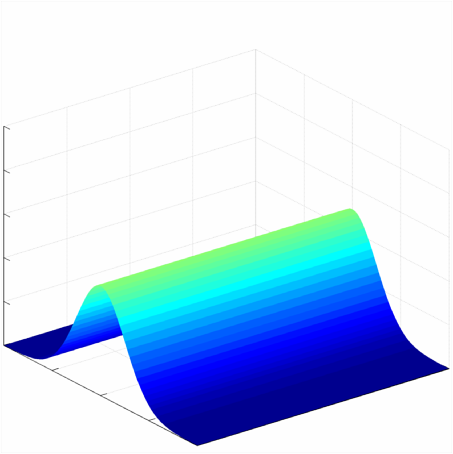
\includegraphics[width=0.2\textwidth]{\additivefigsdir/2d-kernel/additive_kernel_sum_p2} 
& \hspace{-0.4cm} \raisebox{1cm}{+} \hspace{-0.4cm} & 
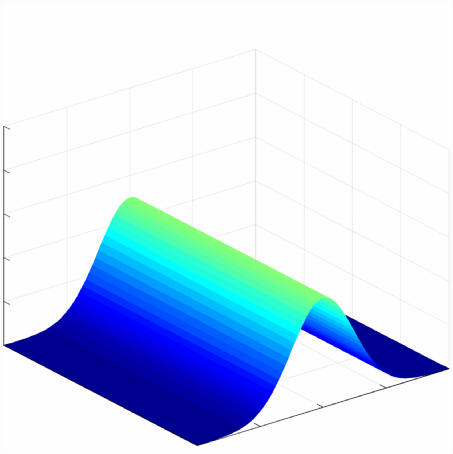
\includegraphics[width=0.2\textwidth]{\additivefigsdir/2d-kernel/additive_kernel_sum_p1} 
& \hspace{-0.4cm} \raisebox{1cm}{=} \hspace{-0.4cm} & 
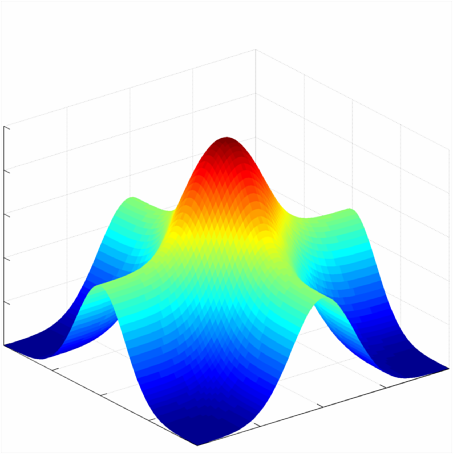
\includegraphics[width=0.2\textwidth]{\additivefigsdir/2d-kernel/additive_kernel} &
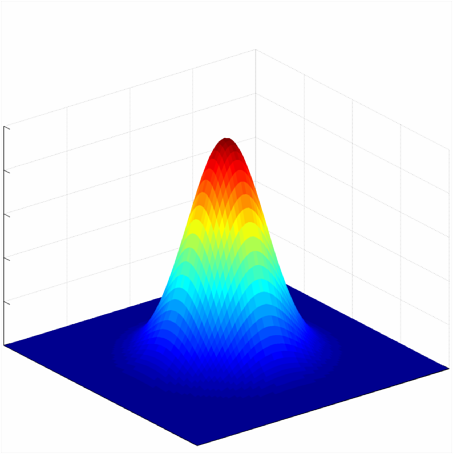
\includegraphics[width=0.2\textwidth]{\additivefigsdir/2d-kernel/sqexp_kernel} \\
$k_1(x_1, x_1')$ & & $k_2(x_2, x_2')$ & & $k_1(x_1,x_1') + k_2(x_2,x_2')$ &$k_1(x_1,x_1')k_2(x_2,x_2')$ \\
%1D kernel & & 1D kernel & & 1st order kernel & 2nd order kernel \\ 
%& & & & & \\
%(Second Order) & & & & & Additive Kernel \\
&&&&& \\
\large $\downarrow$ & & \large $\downarrow$ & & \large $\downarrow$ & \large $\downarrow$  \\
\hspace{-0.2cm}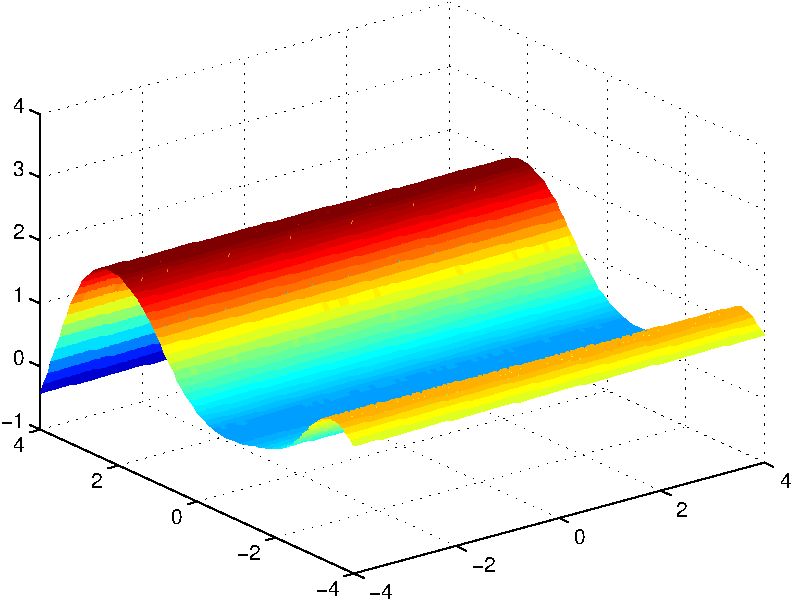
\includegraphics[width=0.2\textwidth]{\additivefigsdir/2d-kernel/additive_kernel_draw_sum_p1}
& \hspace{-0.4cm} \raisebox{1cm}{+} \hspace{-0.4cm} & 
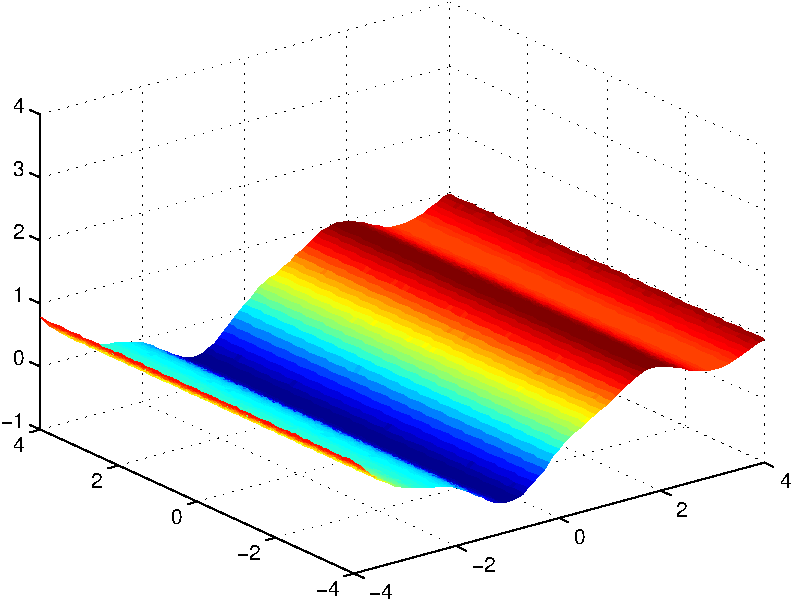
\includegraphics[width=0.2\textwidth]{\additivefigsdir/2d-kernel/additive_kernel_draw_sum_p2}
& \hspace{-0.4cm} \raisebox{1cm}{=} \hspace{-0.4cm} &
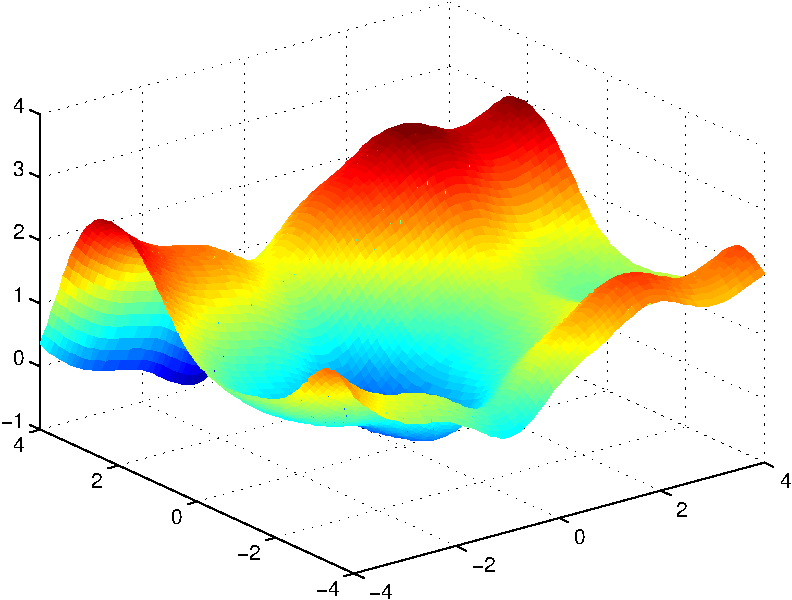
\includegraphics[width=0.2\textwidth]{\additivefigsdir/2d-kernel/additive_kernel_draw_sum} &
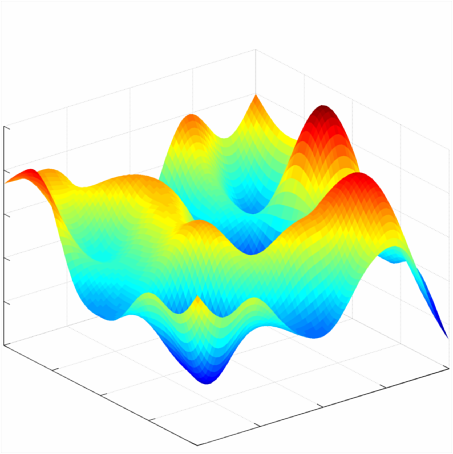
\includegraphics[width=0.2\textwidth]{\additivefigsdir/2d-kernel/sqexp_draw} \\
$f_1 \sim \GP\left(0, k_1\right)$ & & $f_2 \sim \GP\left(0, k_2\right)$ & & $f_1(x_1) + f_2(x_2)$ & $f(x_1, x_2)$ \\
%draw from & & draw from & & draw from & draw from\\
%1D GP prior & & 1D GP prior & & 1st order GP prior & 2nd order GP prior\\
%Draw from product kernel GP prior & Draw from additive kernel GP prior\\
\end{tabular}
\caption[Additive kernels correspond to additive functions]{Top left: An additive kernel is simply a sum of kernels.  Bottom left:  A draw from an additive kernel corresponds to a sum of draws from \gp{}s with the corresponding kernels.  Top right: a product kernel is a product of kernels.  Bottom right:  A draw from a product kernel does not correspond to a product of draws from the corresponding kernels.
%In this example, both kernels are composed of one dimensional squared-exponential kernels, but this need not be the case in general.
}
\label{fig:kernels}
\end{figure}

Figure \ref{fig:kernels} compares, for two-dimensional functions, a first-order additive kernel with a second-order kernel.



\subsubsection{Long-range extrapolation through additivity}

Because additive kernels can discover non-local structure in data, they are exceptionally well-suited to problems where local interpolation fails.  
%[Would this make them good for nonstationary noise?]
\begin{figure}[h]
\centering
\begin{tabular}{cccc}
\hspace{-0.1in}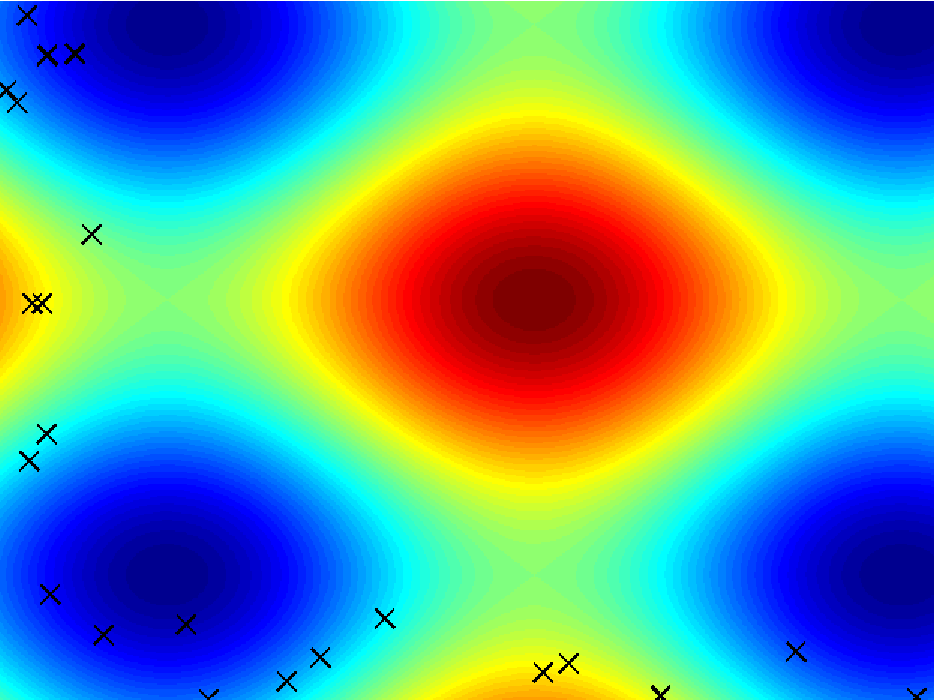
\includegraphics[width=0.24\textwidth]{\additivefigsdir/1st_order_censored_truth.pdf} &
\hspace{-0.1in}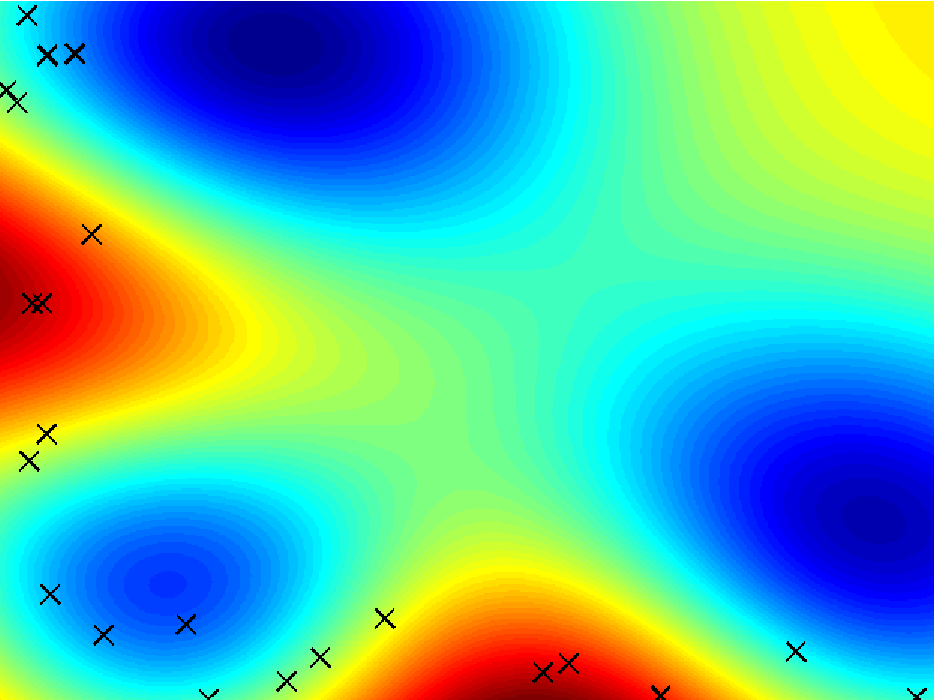
\includegraphics[width=0.24\textwidth]{\additivefigsdir/1st_order_censored_ard.pdf}&
\hspace{-0.1in}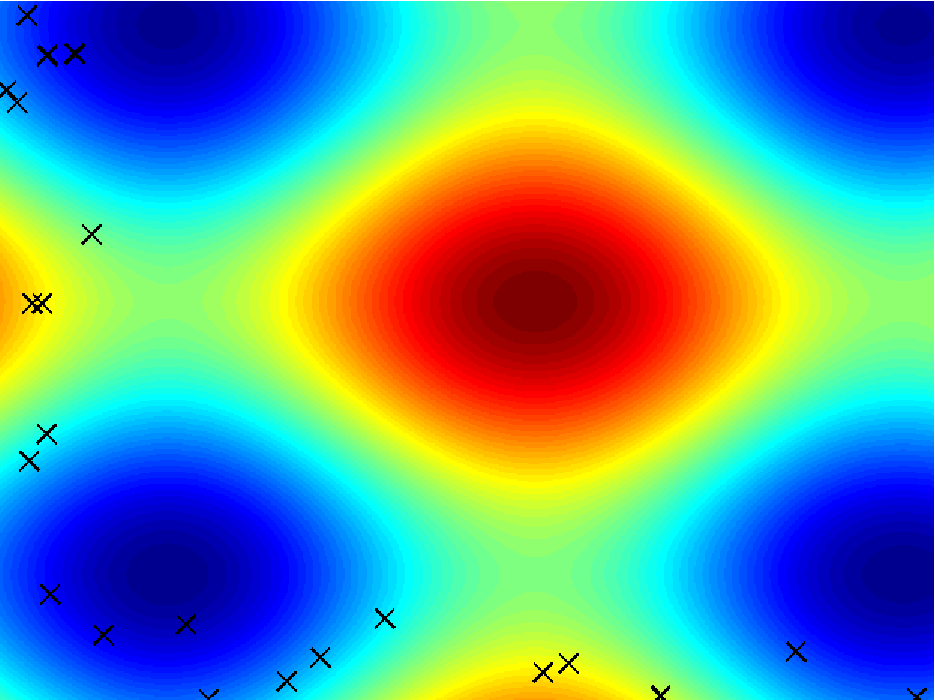
\includegraphics[width=0.24\textwidth]{\additivefigsdir/1st_order_censored_add.pdf}& 
\hspace{-0.1in}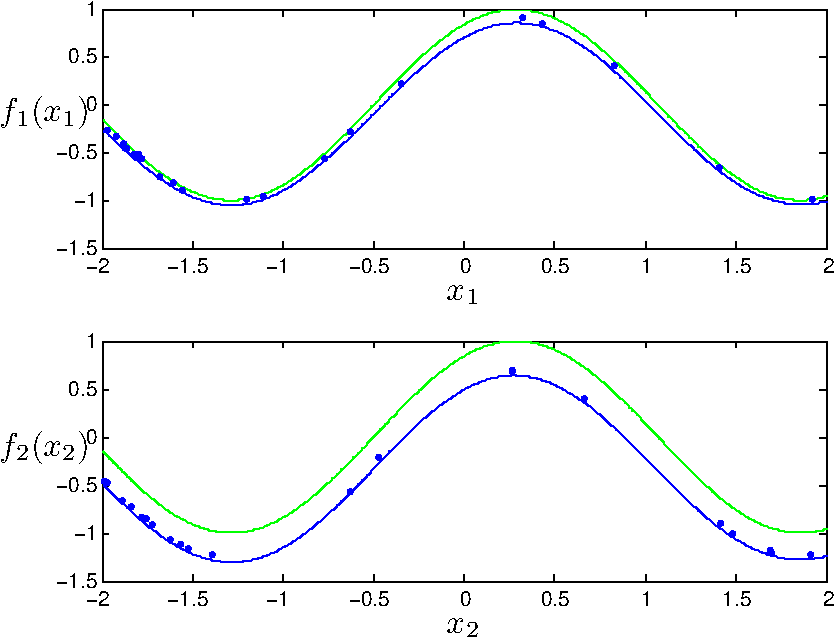
\includegraphics[width=0.24\textwidth]{\additivefigsdir/1st_order_censored_d1d2.pdf}\\ 
True Function & Squared-exp GP & Additive GP & Additive GP \\
 \& data locations & posterior mean & posterior mean & 1st-order functions\\
%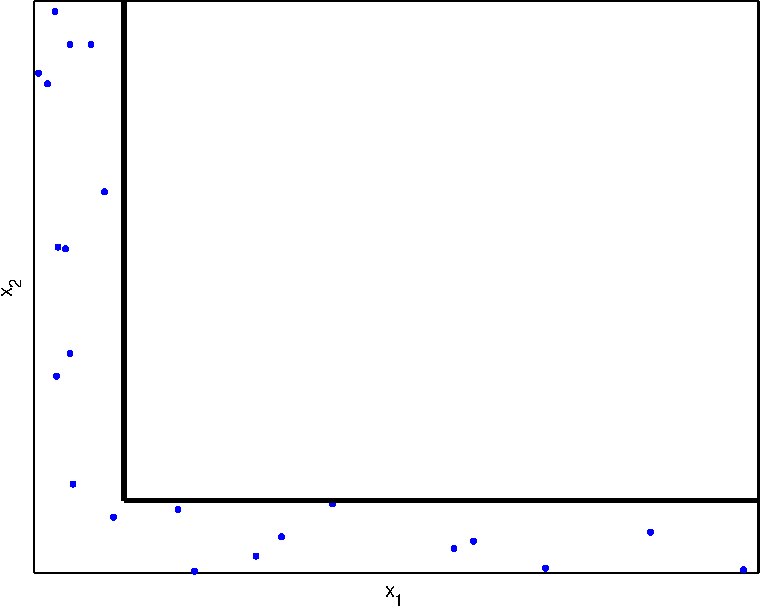
\includegraphics[width=0.3\textwidth]{\additivefigsdir/1st_order_censored_data.pdf} &
%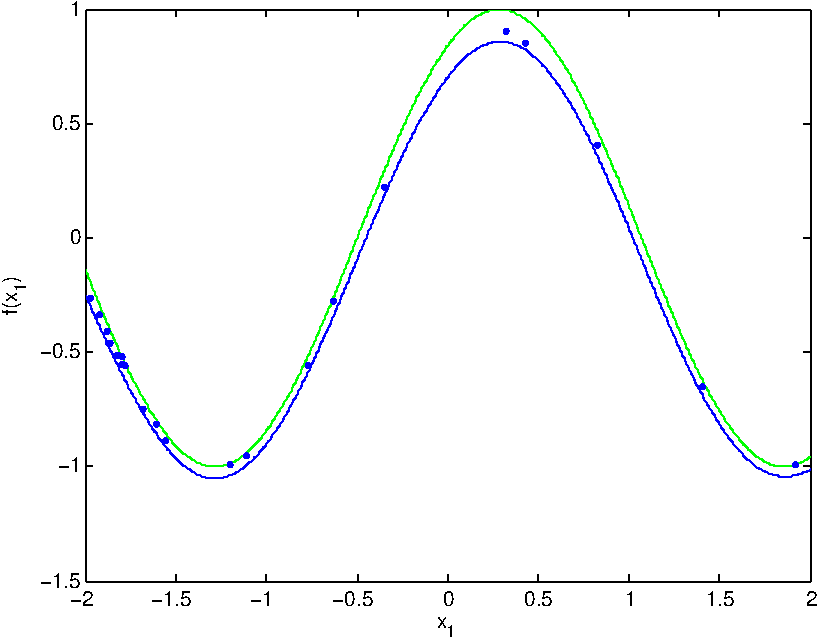
\includegraphics[width=0.3\textwidth]{\additivefigsdir/1st_order_censored_d1.pdf}&
%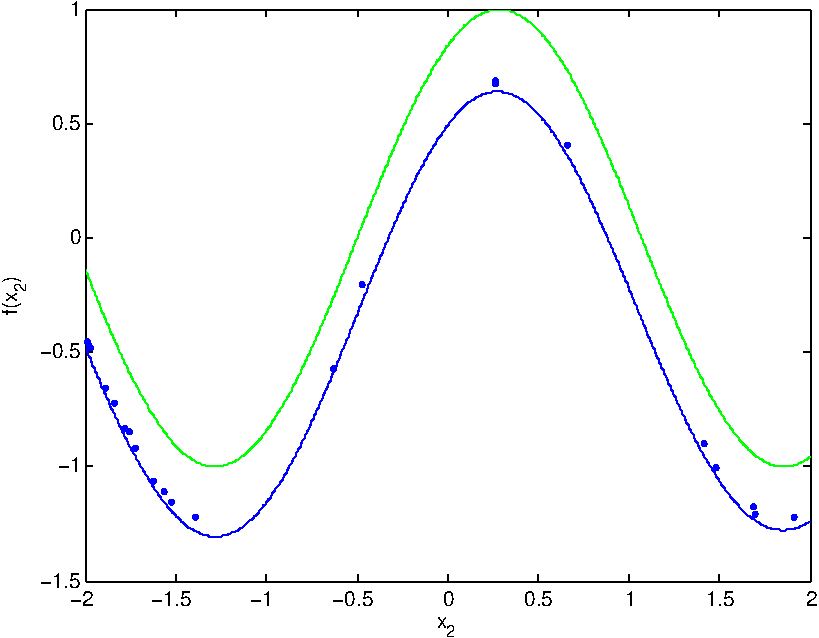
\includegraphics[width=0.3\textwidth]{\additivefigsdir/1st_order_censored_d2.pdf}\\
%Training Data Locations & Estimated 1D $f(x_1)$ & Estimated 1D $f(x_2)$ \\
\end{tabular}
\caption[Long-range inference in functions with additive structure]
{Long-range inference in functions with additive structure.%  The additive GP is able to discover the additive pattern, and use it to fill in a distant mode.  The ARD kernel can only interpolate, and thus predicts the mean in locations missing data.
}
\label{fig:synth2d}
\end{figure}
%Figure \ref{fig:synth2d} shows a simple experiment demonstrating the ability of additive kernels to discover low-order structure, and to exploit that structure to make predictions about unseen combinations of inputs.
Figure \ref{fig:synth2d} shows a dataset which demonstrates this feature of additive GPs, consisting of data drawn from a sum of two axis-aligned sine functions.  The training set is restricted to a small, L-shaped area; the test set contains a peak far from the training set locations.  The additive GP recovered both of the original sine functions (shown in green), and inferred correctly that most of the variance in the function comes from first-order interactions.  The ability of additive GPs to discover long-range structure suggests that this model may be well-suited to deal with covariate-shift problems.






\section{Structure through Multiplication}

Multiplying kernels allows us to account for interactions between different input dimensions or different notions of similarity. 
For instance, in multidimensional data, the multiplicative kernel $\SE_1 \times \SE_3$ represents a smoothly varying function of dimensions 1 and 3 which is not constrained to be additive.
In univariate data, multiplying a kernel by \kSE{} gives a way of converting global structure to local structure. 
For example, $\Per$ corresponds to globally periodic structure, whereas $\Per \times \SE$ corresponds to locally periodic structure, as shown in row 1 of figure~\ref{fig:kernels}.

Many architectures for learning complex functions, such as convolutional networks \cite{lecun1989backpropagation} and sum-product networks \cite{poon2011sum}, include units which compute AND-like and OR-like operations.
Composite kernels can be viewed in this way too. A sum of kernels can be understood as an OR-like operation: two points are considered similar if either kernel has a high value.
Similarly, multiplying kernels is an AND-like operation, since two points are considered similar only if both kernels have high values.
Since we are applying these operations to the similarity functions rather than the regression functions themselves, compositions of even a few base kernels are able to capture complex relationships in data which do not have a simple parametric form.

From a kernel point of view,

if $k_1(\vx, \vx') = \phi_1(\vx)\tra \phi_1(\vx')$ and $k_2 = \phi_2(\vx)\tra \phi_2(\vx')$
then
%
\begin{align}
k_1(\vx, \vx') \times k_2(\vx, \vx') = \left[\phi_1(\vx) + \phi_2(\vx)\right]\tra \left[ \phi_1(\vx') + \phi_2(\vx') \right]
\end{align}

In other words, the features of $k_1 \times k_2$ are the cartesian product (all possible combinations) of the original sets of features.


\subsection{Multiplying with constant functions}

If we wish to model a function that's been multiplied by some fixed function $a(x)$, this can be easily achieved by multiplying the kernel by $a(\vx) a(\vx')$.

This is why it is common practice to assume zero mean, since marginalizing over an unknown mean function can be equivalently expressed as a zero-mean \gp{} with a new kernel.




\subsection{Signal versus noise}

In most derivations of Gaussian processes, the model is given as $y = f + \epsilon$, where $\epsilon \simiid \Nt{0}{\sigma^2_{\textnormal{noise}}}$.

However, $\epsilon$ can equivalently be thought of as another Gaussian process, and so this model can be written as one in which $f \sim \GP\left(0, k + \delta \right)$.  The lack of distinction between the noise model and the model of the signal raises the larger question:  Which part of a model represents signal, and which represents noise?

Our answer is: \emph{it depends on what you want to do with the model}.  For example: often, we don't care about the short-term variations in a function, and only in the long-term trend.  However, in many other cases, we with to de-trend our data to see more clearly how much a particular part of the signal deviated from normal.

\subsubsection{Student's $t$ processes}

One shortcoming of the




\section{Expressing Symmetries}


When modeling functions, encoding known symmetries greatly aids learning and prediction.  We demonstrate that in nonparametric regression, many types of symmetry can be enforced through operations on the covariance function.  These symmetries can be composed to produce nonparametric priors on functions whose domains have interesting topological structure such as spheres, torii, and M\"{o}bius strips.  We demonstrate that marginal likeihood an be used to automatically search over such structures.

Joint work with David Reshef, Roger Grosse, Joshua B. Tenenbaum



%connected Riemannian manifold

It is well-known that the properties of the functions we wish to model can be expressed mainly through the covariance function \cite{rasmussen38gaussian}.



In this section, we give recipes for expressing several classes of symmetries.  Later, we will show how these can be combined to produce more interesting structures.

\paragraph{Periodicity}
Given $D$ dimensions, we can enforce rotational symmetry on any subset of the dimensions:
%
\begin{align}
f(x) = f( x_i + k \tau_i) \quad \forall k \in \mathbb{Z}
\end{align}
%
by the applying a kernel between pairs transformed coordinates $\sin(x), \cos(x)$:
%
\begin{align}
k_{\textnormal{periodic}}(x, x') = k(\sin(x), \cos(x), \sin(x'), \cos(x'))
\end{align}
%
We can also apply rotational symmetry repeatedy to a single dimension.

\paragraph{Reflective Symmetry along an axis}
we can enforce the symmetry
\begin{align}
f(x) = f( -x)
\end{align}
%
by the kernel transform
%
\begin{align}
k_{\textnormal{symm arg1}}(x, x') & = k(x, x') + k(x, -x') + k(-x, x') + k(-x, -x')
\end{align}

\paragraph{Reflective Symmetry along a diagonal}
We can enforce symmetry between any two dimensions:
%
\begin{align}
f(x, y) = f( y, x)
\end{align}
%
by two methods:  In the additive method, we transform the kernel by:
%
\begin{align}
k_{\textnormal{reflect add}}(x, y, x', y') 
 = k(x, y, x', y') + k(x, y, y', x')
 + k(y, x, x', y') + k(y, x, y', x')
\end{align}
or by
\begin{align}
k_{\textnormal{reflect min}}(x, y, x', y') = k( & \min(x, y), \max(x,y), % \nonumber \\ & 
\min(x', y'), \max(x',y') )
\end{align}
however, the second method will in general lead to non-differentiability along $x = y$.  Figure \ref{fig:add_vs_min} shows the difference.

\begin{figure}
\begin{tabular}{cc}
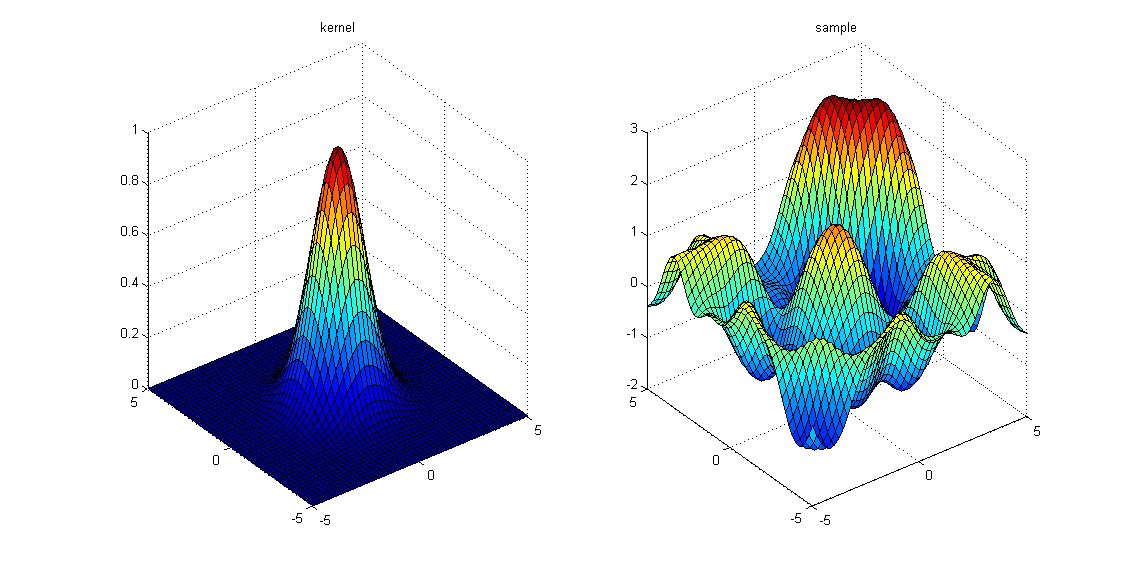
\includegraphics[width=0.33\columnwidth,clip=true,trim=16cm 1cm 3cm 1cm]{\topologyfiguresdir/symmetric-naive} &
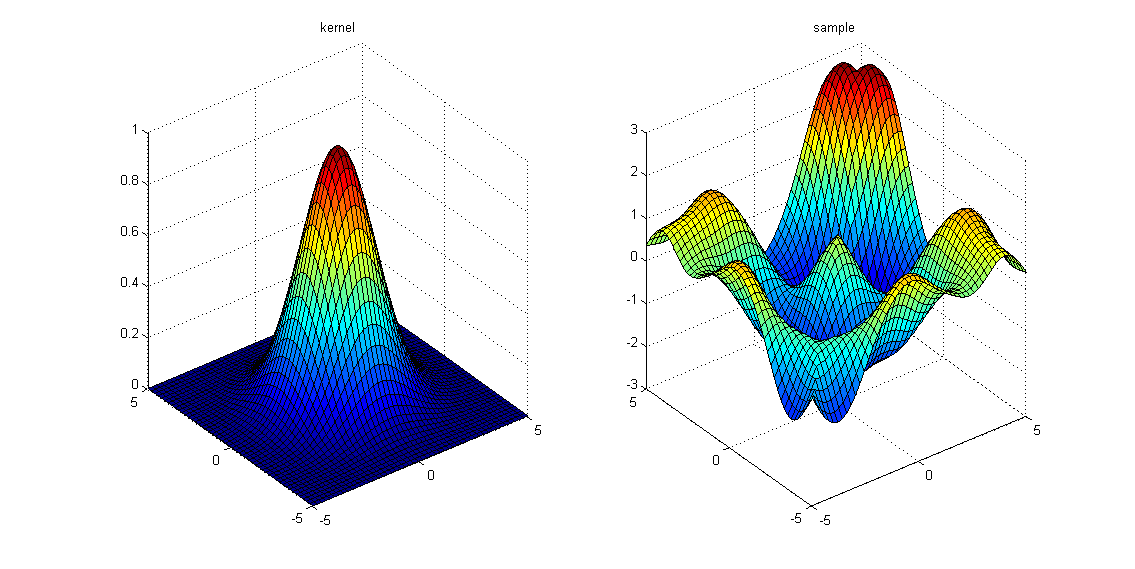
\includegraphics[width=0.33\columnwidth,clip=true,trim=16cm 1cm 3cm 1cm]{\topologyfiguresdir/symmetric-projection} \\
Additive method & min method
\end{tabular}
\caption[Two ways to introduce symmetry]{An illustration of two methods of introducing symmetry: The additive method or the min method.  The additive method has half the marginal variance away from $y = x$, but the min method introduces a non-differentiable seam along $y = x$.}
\label{fig:add_vs_min}
\end{figure}


%\paragraph{Spherical Symmetry}

%We can also enforce that a function expresses the symmetries obeyed by $n-spheres$ by simply transforming a set of $n - 1$ coordinates by:
%
%\begin{align}
%x_1 & = \cos(\phi_1) \nonumber \\
%x_2 & = \sin(\phi_1) \cos(\phi_2) \nonumber \\
%x_3 & = \sin(\phi_1) \sin(\phi_2) \cos(\phi_3) \nonumber \\
%& \vdots \nonumber \\
%x_{n-1} & = \sin(\phi_1) \cdots \sin(\phi_{n-2}) \cos(\phi_{n-1}) \nonumber \\
%x_n & = \sin(\phi_1) \cdots \sin(\phi_{n-2}) \sin(\phi_{n-1})
%\end{align}

%\cite{flanders1989}

\subsection{Parametric embeddings}

In general, we can always enforce the symmetries obeyed by a given surface by finding a parametric embedding to that surface.  However, it is not clear how to do this in general without introducing unnecessary 


%It is possible to construct

%Because then one dimension would be special.









\section{How to generate 3D shapes with a given topology}

First create a mesh in 2d.  Then draw 3 independent functions from a GP prior with the relevant symmetries encoded in the kernel.  Then, map the 2d points making up the mesh through those 3 functions to get the 3D  coordinates of each point on the mesh.

This is similar in spirit to the GP-LVM model \cite{lawrence2005probabilistic}, which learns an embedding of the data into a low-dimensional space, and constructs a fixed kernel structure over that space.

\begin{figure}
\begin{tabular}{ccc}
Manifold $( \SE_1 \times \SE_2 )$  & Cylinder $( \SE_1 \times \Per_2 )$ & Toroid $( \Per_1 \times \Per_2 )$\\
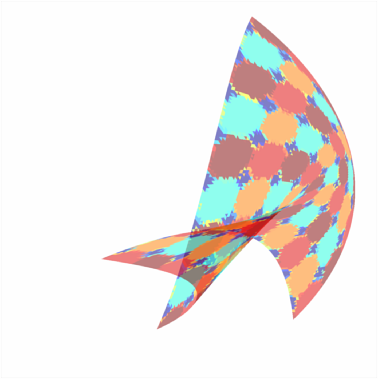
\includegraphics[width=0.33\columnwidth]{\topologyfiguresdir/manifold} &
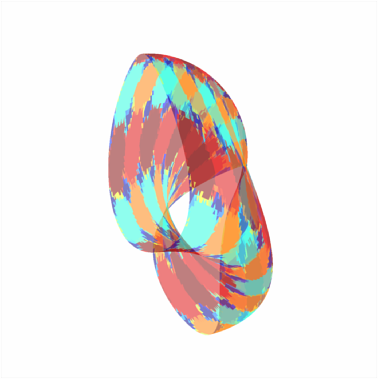
\includegraphics[width=0.33\columnwidth]{\topologyfiguresdir/cylinder} &
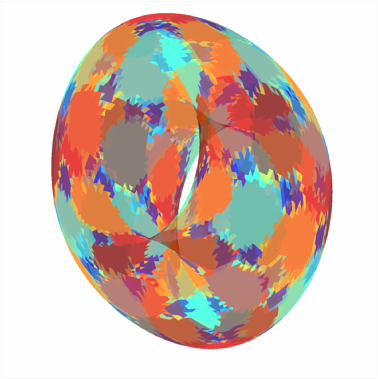
\includegraphics[width=0.33\columnwidth]{\topologyfiguresdir/torus} \\
\end{tabular}
\caption[Generating 2D manifolds with different topological structures]{Generating 2D manifolds with different topological structures.  By enforcing that the functions mapping from $\mathbb{R}^2$ to $\mathbb{R}^3$ obey the appropriate symmetries, the surfaces created have the corresponding topologies, ignoring self-intersections.}
\label{fig:gen_surf}
\end{figure}



\subsection{M\"{o}bius strips}

A prior on functions on M\"{o}bius strips can be achieved by enforcing the symmetries:
%
\begin{align}
f(x, y) & = f( x, y + \tau_y) \\
f(x, y) & = f( x + \tau_x, y)  \\
f(x, y) & = f( y, x )
\end{align}

If we imagine moving along the edge of a M\"{o}bius strip, that is equivalent to moving along a diagonal in the function generated.
Figure \ref{fig:mobius} shows this.
%
\begin{figure}
\begin{tabular}[t]{m{.33\columnwidth} m{.33\columnwidth} m{.33\columnwidth}}
%\begin{columns}
\centering Function on M\"{o}bius strip &
M\"{o}bius manifold & 
Sudanese M\"{o}bius strip \\
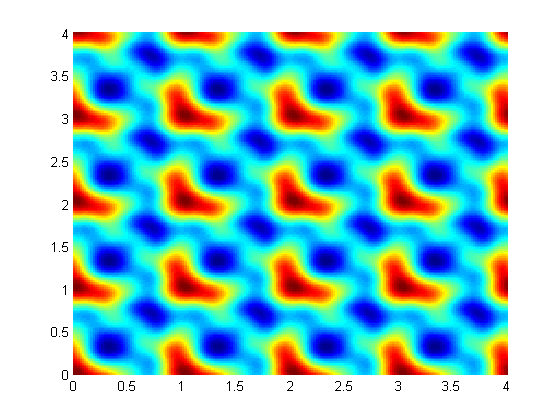
\includegraphics[width=0.3\columnwidth, height=0.3\columnwidth, clip=true,trim=3cm 2cm 2cm 2cm]{\topologyfiguresdir/mobius_field} &
%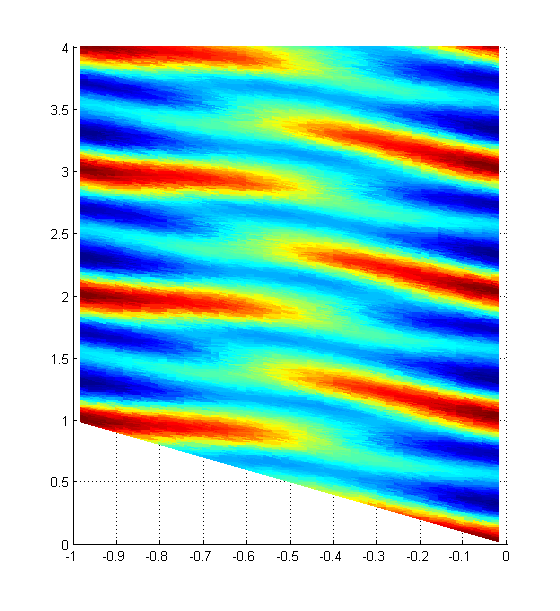
\includegraphics[width=0.45\columnwidth, height=0.45\columnwidth, clip=true,trim=2cm 2cm 2cm 1cm]{\topologyfiguresdir/mobius_regression} \\
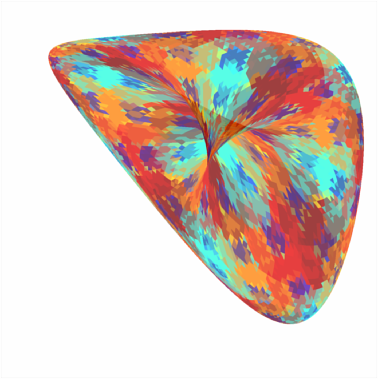
\includegraphics[width=0.3\columnwidth]{\topologyfiguresdir/mobius} &
%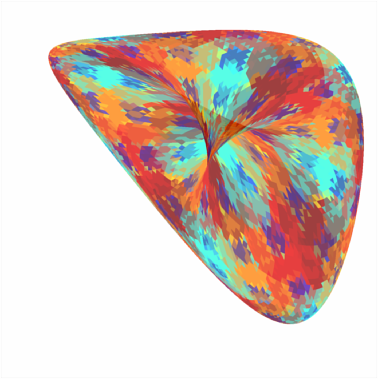
\includegraphics[width=0.33\columnwidth]{\topologyfiguresdir/mobius} 
%\begin{minipage}{0.33\columnwidth}
{\begin{tabular}[t]{p{.3\columnwidth}}
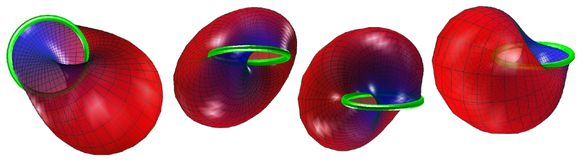
\includegraphics[width=0.3\columnwidth,clip=true,trim=0cm 0cm 10cm 0cm]{\topologyfiguresdir/sudanese-wikipedia}
\\
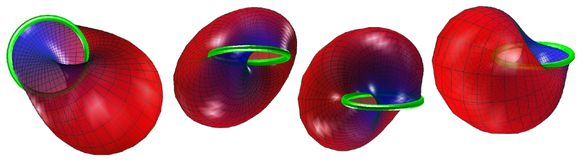
\includegraphics[width=0.3\columnwidth,clip=true,trim=10.55cm 0cm 0cm 0cm]{\topologyfiguresdir/sudanese-wikipedia}
\end{tabular}}
%\end{minipage}
\end{tabular}
\caption[Generating M\"{o}bius strips]{Generating M\"{o}bius strips.  By enforcing that the functions mapping from $\mathbb{R}^2$ to $\mathbb{R}^3$ obey the appropriate symmetries, the surfaces created have topology corresponding to a M\"{o}bius strip. TODO: Talk about Sudanese representation.}
\label{fig:mobius}
\end{figure}
%
The second example is doesn't resemble a typical M\"{o}bius strip because the edge of the mobius strip is in a geometric circle.  This kind of embedding is resembles the Sudanese M\"{o}bius strip [cite].

Another classic example of a function living on a Mobius strip is the auditory quality of 2-note intervals.  The harmony of a pair of notes is periodic (over octaves) for each note, and the 


\section{Discrete data}

Kernels can be defined over all types of data structures: Text, images, matrices, and even kernels . Coming up with a kernel on a new type of data used to be an easy way to get a NIPS paper.

\subsection{Categorical variables}

There is a simple way to do GP regression over categorical variables. Simply represent your categorical variable as a by a one-of-k encoding. This means that if your number ranges from 1 to 5, represent that as 5 different data dimensions, only one of which is on at a time. 

Then, simply put a product of SE kernels on those dimensions. This is the same as putting one SE ARD kernel on all of them. The lengthscale hyperparameter will now encode whether, when that coding is active, the rest of the function changes. If you notice that the estimated lengthscales for your categorical variables is short, your model is saying that it's not sharing any information between data of different categories. 



\section{Examples}

\subsection{Computing molecular energies}

\begin{figure}
\begin{center}
  \begin{tikzpicture}

%\pgfmathsetmacro{\r}{3cm}
%\pgfmathsetmacro{\ho}{70}
%\pgfmathsetmacro{\ht}{30}
\newcommand{\radius}{3}
\newcommand{\hone}{120}
\newcommand{\htwo}{70}
\newcommand{\hthree}{30}

	\coordinate (O) at (0, 0);
	\coordinate (left) at ({\radius*cos(\hone)}, {\radius*sin(\hone)});
	\coordinate (right) at ({\radius*cos(\htwo)}, {\radius*sin(\htwo)});
	\coordinate (zero) at ({\radius*cos(\hthree)}, {\radius*sin(\hthree)});

	\draw[fill] (left) circle (2pt);
	\draw (left) node[below, left] {H};
	
	\draw[fill] (right) circle (2pt);
	\draw (right) node[right] {H};

	\draw[fill] (zero) circle (2pt);
	\draw (zero) node[right] {H};

	\draw[fill] (O) circle (3pt);
	\draw (O) node[below] {C};

	\draw (left) -- (O);
	\draw (right) -- (O);
	\draw (zero) -- (O);

	\begin{scope}
	\path[clip] (O) -- (right) -- (zero);
	\fill[red, opacity=0.5, draw=black] (O) circle (2);
	\node at ($(O)+(50:1.6)$) {$\theta_1$};	
	\end{scope}
	
	\begin{scope}
	\path[clip] (O) -- (left) -- (right);
	\fill[green, opacity=0.5, draw=black] (O) circle (1.8);
	\node at ($(O)+(90:1.4)$) {$\theta_2$};	
	\end{scope}	
	
  \end{tikzpicture}
\end{center}
\caption[The energy of a molecular configuration obeys the same symmetries as a M\"{o}bius strip]{An example of a function expressing the same symmetries as a M\"{o}bius strip in two of its arguments.  The energy of a molecular configuration $f(\theta_1, \theta_2)$ depends only on the relative angles between atoms, and because each atom is indistiguishable, is invariant to permuting the atoms. }
\label{fig:molecule}
\end{figure}

Figure \ref{fig:molecule} gives one example of a function which obeys the same symmetries as a M\"{o}bius strip, in some subsets of its arguments.


\subsection{Translation invariance in images}

Most models of images are invariant to spatial translations [cite convolution nets].  Similarily, most models of sounds are also invariant to translation through time.

Note that this sort of translational invariance is completely distinct from the stationarity properties of kernels used in Gaussian process priors.  A stationary kernel implies that the prior is invariant to translations of the entire training and test set.

We are discussing here a discretized input space (into pixels or the audio equivalent), where the input vectors have one dimension for every pixel.  We are interested in creating priors on functions that are invariant to shifting a signal along its pixels:
%
\begin{align}
f \Bigg( \raisebox{-2.5ex}{ 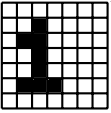
\includegraphics[width=1cm]{\topologyfiguresdir/grid2} } \Bigg) 
= f \Bigg( \raisebox{-2.5ex}{ 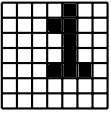
\includegraphics[width=1cm]{\topologyfiguresdir/grid3} } \Bigg)
\end{align}

Translational invariance in this setting is equivalent to symmetries between dimensions in the input space.

This prior can be achieved in one dimension by using the following kernel transformation:
%
\begin{align}
k \left( (x_1, x_2, \dots, x_D ), (x_1', x_2', \dots, x_D' ) \right) & = %\nonumber \\
\sum_{i=1}^D \prod_{j=1}^D k( x_j, x_{ i + j \textnormal{mod $D$} }' )
\end{align}
%
Edge effects can be handled either by wrapping the image around, or by padding it with zeros.

\paragraph{Convolution} The resulting kernel could be called a \emph{discrete convolution kernel}.  For an image with $R, C$ rows and columns, it can also be written as:
%
\begin{align}
k_{\textnormal{conv}} \left( (x_{11}, x_{12}, \dots, x_{RC} ), (x_{11}', x_{12}', \dots, x_{RC}' ) \right) = % \nonumber \\
%\sum_{i=-L}^L \sum_{j=-L}^L k\left( (x_{1+i,1+j}, x_{1+i,2+j} , \dots, x_{R+i,C+j} ), (x_{1+i,1+j}', x_{1+i,2+j}' , \dots, x_{R+i,C+j}' ) \right)
\sum_{i=-L}^L \sum_{j=-L}^L k\left( \vx, T_{ij}(\vx') \right)
\end{align}
%
where $T_{ij}(\vx)$ is the operator which replaces each $x_{mn}$ with $x_{m+i, n+j}$.  Thus we are simply defining the covariance between two images to be the sum of all covariances between all relative translations of the two images.  We can also normalize the kernel by pre-multiplying it with $\sqrt{k_{\textnormal{conv}}(\vx, \vx) k_{\textnormal{conv}}(\vx', \vx') }$.

%$f \left( 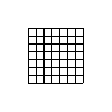
\begin{tikzpicture} \draw[step=0.1,black,thin] (0.3,0.3) grid (1,1); \end{tikzpicture} \right)$



Is there a pathology of the additive construction that appears in the limit?

\subsection{Max-pooling}
What we'd really like to do is a max-pooling operation.  However, in general, a kernel which is the max of other kernels is not PSD [put counterexample here?].  Is the max over co-ordinate switching PSD?

\section{Related Work}
\label{sec:related_work}

\paragraph{Invariances in Gaussian processes}
\cite{Invariances13} show that, for Gaussian processes, with probability one, $f(\vx) = f(T(\vx))$ if and only if $k(x, x') = k(x, T(x'))$.








\section{Deep kernels}
\label{sec:deep_kernels}


\cite{NIPS2005_424} showed that kernel machines have limited generalization ability when they use a local kernel such as the squared-exp.
However, many interesting non-local kernels can be constructed which allow non-trivial extrapolation.
For example, periodic kernels can be viewed as a 2-layer-deep kernel, in which the first layer maps $x \rightarrow [\sin(x), \cos(x)]$, and the second layer maps through basis functions corresponding to the \humble{SE} kernel.

%In addition to analyzing \MLP{}s with random weights, we can also analyze fixed feature mappings with different connectivity architectures.
 
Can we construct other useful kernels by composing fixed feature maps several times, creating deep kernels?  \citet{cho2012kernel} constructed kernels of this form, repeatedly applying multiple layers of feature mappings.
%Given a kernel $k_1(\vx, \vx') = \hPhi(\vx) \tra \hPhi(\vx')$, 
We can compose the feature mapping of two kernels:
\begin{align}
k_{1}(\vx, \vx') & = \hPhi_1(\vx) \tra \hPhi_1(\vx') \\
k_{2}(\vx, \vx') & = \hPhi_2(\vx) \tra \hPhi_2(\vx') \\
\left( k_1 \circ k_2 \right)(\vx, \vx') & = k_2 \left(\hPhi_1(\vx), \hPhi_1(\vx') \right) \\
& = \left[ \hPhi_2 \left( \hPhi_1(\vx) \right)\right] \tra \hPhi_2 \left(\hPhi_1(\vx') \right) 
\end{align}

Composing the squared-exp kernel with any implicit mapping $\hPhi(\vx)$ has a simple closed form:
%, this composition operation has a closed form for any starting kernel:% for any set of starting features $\hPhi_n(\vx)$:
%
\begin{align}
%k_1(\vx, \vx') & = \exp \left( -\frac{1}{2} ||\vx - \vx'||_2^2 \right) \\
k_{L+1} \left( \vx, \vx' \right) & = k_{SE} \left( \hPhi(\vx), \hPhi(\vx') \right) =  \\
%& = \left( \hPhi^{SE} \left(\hPhi^{1}(\vx) \right) \right) \tra \hPhi^{SE} \left( \hPhi^{1}(\vx') \right) \\
& = \exp \left( -\frac{1}{2} || \hPhi(\vx) - \hPhi(\vx')||_2^2 \right) \nonumber\\
%k_{n+1}(\vx, \vx') 
%& = \exp \left( -\frac{1}{2} \sum_i \left[ \hphi_n^{(i)}(\vx) - \hphi_n^{(i)}(\vx') \right]^2 \right) \\
& = \exp\left ( -\frac{1}{2} \left[ \hPhi(\vx) \tra \hPhi(\vx) - 2 \hPhi(\vx) \tra \hPhi(\vx') + \hPhi(\vx') \tra \hPhi(\vx') \right] \right) \nonumber \\
%k_2(\vx, \vx') & = \exp \left( -\frac{1}{2} \left[ \sum_i \hphi_i(\vx)^2 - 2 \sum_i \hphi_i(\vx) \hphi_i(\vx') + \sum_i \hphi_i(\vx')^2 \right] \right) \\
%k_{n+1}(\vx, \vx') 
& = \exp \left( -\frac{1}{2} \left[ k_{L}(\vx, \vx) - 2 k_{L}(\vx, \vx') + k_{L}(\vx', \vx') \right] \right) \nonumber
%k_{n+1}(\vx, \vx') 
%& = \exp \left( k_1(\vx, \vx') - 1 \right) \qquad \textnormal{(if $k_1(\vx, \vx) = 1$)} \nonumber
\end{align}
%
%\begin{figure}
%\centering
%\begin{tabular}{ccc}
%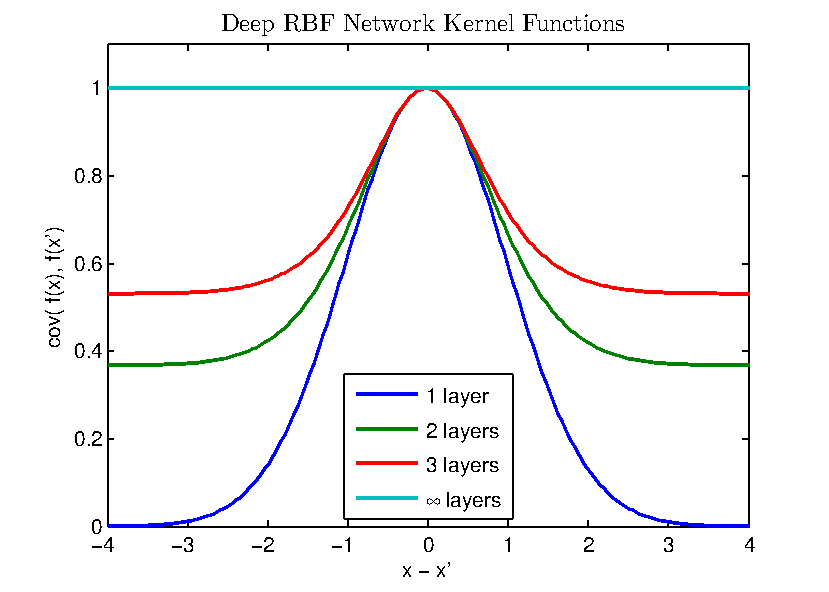
\includegraphics[width=0.5\columnwidth, clip, trim = 0cm 0cm 0cm 0.61cm]{\deeplimitsfiguresdir/deep_kernel} &
%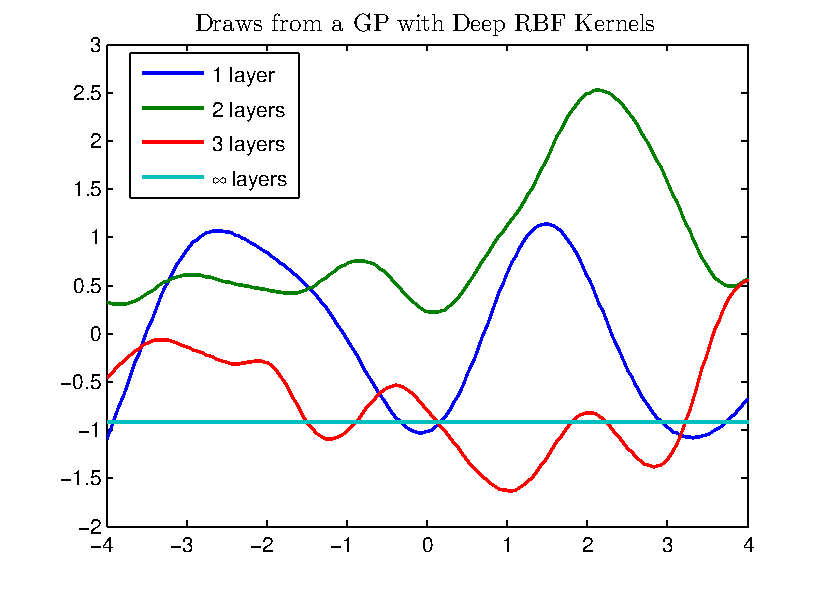
\includegraphics[width=0.5\columnwidth, clip, trim = 0cm 0cm 0cm 0.61cm]{\deeplimitsfiguresdir/deep_kernel_draws} \\
%Kernel derived from iterated feature transforms & Draws from the corresponding kernel
%\end{tabular}
%\caption{A degenerate kernel produced by repeatedly applying a feature transform.}
%\label{fig:deep_kernel}
%\end{figure}
%
%Thus, if $k_1(x,y) = e^{-||x - y||2}$, then the two-layer kernel is simply $k_2(x,y) = e^{k_1(x, y) - 1}$.  This formula is true for every layer: $k_{n+1}(x,y) = e^{k_n(x, y) - 1}$.
%
%Note that nothing in this derivation depends on details of $k_n$, except that $k_n( \vx, \vx) = 1$.
%Note that this result holds for any base kernel $k_n$, as long as $k_n( \vx, \vx) = 1$.
%  Because this is true for $k_2$ as well, this recursion holds in general, and we have that $k_{n+1}(x,y) = e^{k_n(x, y) - 1}$.  
Thus, we can express $k_{L+1}$ exactly in terms of $k_L$.

\paragraph{Infinitely deep kernels}
What happens when we repeat this composition of feature maps many times, starting with the squared-exp kernel?  In the infinite limit, this recursion converges to $k(\vx,\vx') = 1$ for all pairs of inputs, which corresponds to a prior on constant functions $f(\vx) = c$.

%Figure \ref{fig:deep_kernel_connected} shows this kernel at different depths, including the degenerate limit.  
%
%One interpretation of why repeated feature transforms lead to this degenerate prior is that each layer can only lose information about the previous set of features.  
%In the limit, the transformed features contain no information about the original input $\vx$.  Since the function doesn't depend on its input, it must be the same everywhere.

\paragraph{A non-degenerate construction}

As before, we can overcome this degeneracy by % following a suggestion from \cite{neal1995bayesian}, we 
connecting the inputs $\vx$ to each layer.  To do so, we simply augment the feature vector $\hPhi_{L}(\vx)$ with $\vx$ at each layer: 
%
\begin{align}
%k_1(\vx, \vx') & = \exp \left( -\frac{1}{2} ||\vx - \vx'||_2^2 \right) \\
 k_{L+1}(\vx, \vx') % = \nonumber\\
& = \exp \left( -\frac{1}{2} \left|\left| \left[ \! \begin{array}{c} \hPhi_{L}(\vx) \\ {\color{blue} \vx} \end{array} \! \right]  - \left[ \! \begin{array}{c} \hPhi_{L}(\vx') \\ {\color{blue} \vx'} \end{array} \! \right] \right| \right|_2^2 \right) \nonumber \\
%k_{n+1}(\vx, \vx') 
%& = \exp \left( -\frac{1}{2} \sum_i \left[ \hphi_i(\vx) - \hphi_i(\vx') \right]^2 -\frac{1}{2} || \vx - \vx' ||_2^2 \right) \\
%k_{n+1}(\vx, \vx') & = \exp\left ( -\frac{1}{2} \sum_i \left[ \hphi_i(\vx)^2 - 2 \hphi_i(\vx) \hphi_i(\vx') + \hphi_i(\vx')^2 \right]  -\frac{1}{2} || \vx - \vx' ||_2^2 \right) \\
%k_2(\vx, \vx') & = \exp \left( -\frac{1}{2} \left[ \sum_i \hphi_i(\vx)^2 - 2 \sum_i \hphi_i(\vx) \hphi_i(\vx') + \sum_i \hphi_i(\vx')^2 \right] \right) \\
%k_2(\vx, \vx') & = \exp \left( -\frac{1}{2} \left[ k_1(\vx, \vx) - 2 k_1(\vx, \vx') + k_1(\vx', \vx') \right] \right) \\
%k_{n+1}(\vx, \vx') 
%& = \exp \left( k_n(\vx, \vx') - 1 -\frac{1}{2} || \vx - \vx' ||_2^2 \right)
& = \exp \Big( -\frac{1}{2} \big[ k_{L}(\vx, \vx) - 2 k_{L}(\vx, \vx') % \nonumber \\ 
 + k_{L}(\vx', \vx') {\color{blue} - || \vx - \vx' ||_2^2} \big] \Big)
\end{align}
%
For the \humble{SE} kernel, this repeated mapping satisfies
\begin{align}
k_\infty(\vx, \vx') - \log \left( k_\infty(\vx, \vx') \right) = 1 + \frac{1}{2} || \vx - \vx' ||_2^2
\end{align}
%
The solution to this recurrence has no closed form, but has a similar shape to the Ornstein-Uhlenbeck covariance ${k_{\textnormal{OU}}(x,x') = \exp( -|x - x'| )}$ with lighter tails.
%
Samples from a \gp{} prior with this kernel are not differentiable, and are locally fractal.
%\item This kernel has smaller correlation than the squared-exp everywhere except at $\vx = \vx'$.  
%\item The tails have the same form as the squared-exp.

\begin{figure}
\centering
\begin{tabular}{cc}
\hspace{-0.3cm}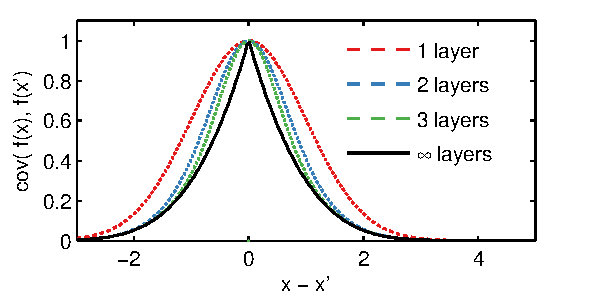
\includegraphics[width=0.5\columnwidth, clip, trim = 0.17cm 0.05cm 0.9cm 0.3cm]{\deeplimitsfiguresdir/deep_kernel_connected} &
\hspace{-0.5cm}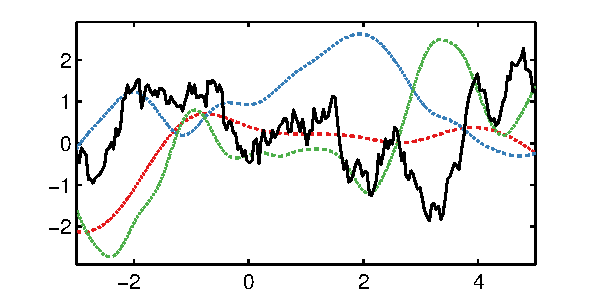
\includegraphics[width=0.5\columnwidth, clip, trim = 0cm 0.1cm 0.9cm 0.35cm]{\deeplimitsfiguresdir/deep_kernel_connected_draws} 
\end{tabular}
\caption[Infinitely deep kernels]{Left:  Input-connected deep kernels.  By connecting the inputs $\vx$ to each layer, the kernel can still depend on its input even after arbitrarily many layers of computation.  Right: GP draws using deep input-connected kernels.  }
\label{fig:deep_kernel_connected}
\end{figure}





%\subsection{A fully-connected kernel}
%However, connecting every layer to every subsequent layer leades to a pathology:
%\begin{align}
%k_1(\vx, \vx') & = \exp \left( -\frac{1}{2} ||\vx - \vx'||_2^2 \right) \\
%k_{n+1}(\vx, \vx') & = \exp \left( -\frac{1}{2} \left|\left| \left[ \! \begin{array}{c} \hPhi_n(\vx) \\ \hPhi_{n-1}(\vx') \end{array} \! \right]  - \left[ \! \begin{array}{c} \hPhi_n(\vx') \\ \hPhi_{n-1}(\vx') \end{array} \! \right] \right| \right|_2^2 \right) \\
%k_{n+1}(\vx, \vx') & = \exp \left( -\frac{1}{2} \sum_i \left[ \hphi^{(i)}_n(\vx) - \hphi^{(i)}_n(\vx') \right]^2 -\frac{1}{2} \sum_i \left[ \hphi^{(i)}_{n-1}(\vx) - \hphi^{(i)}_{n-1}(\vx') \right]^2 \right)\\
%k_{n+1}(\vx, \vx') & = \exp\left ( -\frac{1}{2} \sum_i \left[ \hphi_i(\vx)^2 - 2 \hphi_i(\vx) \hphi_i(\vx') + \hphi_i(\vx')^2 \right]  -\frac{1}{2} || \vx - \vx' ||_2^2 \right) \\
%k_2(\vx, \vx') & = \exp \left( -\frac{1}{2} \left[ \sum_i \hphi_i(\vx)^2 - 2 \sum_i \hphi_i(\vx) \hphi_i(\vx') + \sum_i \hphi_i(\vx')^2 \right] \right) \\
%k_2(\vx, \vx') & = \exp \left( -\frac{1}{2} \left[ k_1(\vx, \vx) - 2 k_1(\vx, \vx') + k_1(\vx', \vx') \right] \right) \\
%k_{n+1}(\vx, \vx') & = \exp \left( k_n(\vx, \vx') - 1 \right) \exp \left( k_{n-1}(\vx, \vx') - 1 \right)
%k_{n+1}(\vx, \vx') & = \prod_{i=1}^n \prod_{j=1}^i \exp \left( k_i(\vx, \vx') - 1 \right)
%\end{align}
%Which has the solution $k_\infty = \delta( \vx = \vx' )$, a white noise kernel.


%\subsection{Connecting every layer to the end}
%There is a fourth possibilty (suggested by Carl), of connecting every layer to the output:
%\begin{align}
%k_n(\vx, \vx') & = \exp \left( -\frac{1}{2} || \hPhi_n(\vx) - \hPhi_n(\vx')||_2^2 \right) \\
%k_{n+1}(\vx, \vx') & = \exp \left( k_n(\vx, \vx') - 1 \right) \\
%k_{L}(\vx, \vx') & = \prod_{i=1}^L \exp \left( k_i(\vx, \vx') - 1 \right)
%\end{align}
%Which also has the solution $k_\infty = \delta( \vx = \vx' )$, a white noise kernel.


\subsection{When are deep kernels useful models?}

Kernels correspond to fixed feature maps, and so kernel learning is an example of implicit representation learning. %can compute %useful representations.
Such feature maps can capture rich structure \citep{DuvLloGroetal13}, and can enable many types of generalization, such as translation and rotation invariance in images \citep{kondor2008group}.
\cite{SalHin08} used a deep neural network to learn feature transforms for kernels, which learn invariances in an unsupervised manner.
%However, any fixed representation is unlikely to be useful for a given problem unless it has been optimized specifically for that problem.
The relatively uninteresting properties of the kernels derived in this section simply reflect the fact that an arbitrary deep computation is not usually a useful representation, unless combined with learning.




\section{Worked example: building a structured kernel for a time-series}

\subsection{Modeling multiple periodicities}

\subsection{Incoportating side-information}

\subsection{Incoportating discrete covariates}

\subsection{Breaking down the predictions, examining different parts of the model}


\outbpdocument{
\bibliographystyle{plainnat}
\bibliography{references.bib}
}


